% Options for packages loaded elsewhere
\PassOptionsToPackage{unicode}{hyperref}
\PassOptionsToPackage{hyphens}{url}
\PassOptionsToPackage{dvipsnames,svgnames,x11names}{xcolor}
%
\documentclass[
  letterpaper,
  DIV=11,
  numbers=noendperiod]{scrartcl}

\usepackage{amsmath,amssymb}
\usepackage{iftex}
\ifPDFTeX
  \usepackage[T1]{fontenc}
  \usepackage[utf8]{inputenc}
  \usepackage{textcomp} % provide euro and other symbols
\else % if luatex or xetex
  \usepackage{unicode-math}
  \defaultfontfeatures{Scale=MatchLowercase}
  \defaultfontfeatures[\rmfamily]{Ligatures=TeX,Scale=1}
\fi
\usepackage{lmodern}
\ifPDFTeX\else  
    % xetex/luatex font selection
\fi
% Use upquote if available, for straight quotes in verbatim environments
\IfFileExists{upquote.sty}{\usepackage{upquote}}{}
\IfFileExists{microtype.sty}{% use microtype if available
  \usepackage[]{microtype}
  \UseMicrotypeSet[protrusion]{basicmath} % disable protrusion for tt fonts
}{}
\makeatletter
\@ifundefined{KOMAClassName}{% if non-KOMA class
  \IfFileExists{parskip.sty}{%
    \usepackage{parskip}
  }{% else
    \setlength{\parindent}{0pt}
    \setlength{\parskip}{6pt plus 2pt minus 1pt}}
}{% if KOMA class
  \KOMAoptions{parskip=half}}
\makeatother
\usepackage{xcolor}
\setlength{\emergencystretch}{3em} % prevent overfull lines
\setcounter{secnumdepth}{-\maxdimen} % remove section numbering
% Make \paragraph and \subparagraph free-standing
\ifx\paragraph\undefined\else
  \let\oldparagraph\paragraph
  \renewcommand{\paragraph}[1]{\oldparagraph{#1}\mbox{}}
\fi
\ifx\subparagraph\undefined\else
  \let\oldsubparagraph\subparagraph
  \renewcommand{\subparagraph}[1]{\oldsubparagraph{#1}\mbox{}}
\fi

\usepackage{color}
\usepackage{fancyvrb}
\newcommand{\VerbBar}{|}
\newcommand{\VERB}{\Verb[commandchars=\\\{\}]}
\DefineVerbatimEnvironment{Highlighting}{Verbatim}{commandchars=\\\{\}}
% Add ',fontsize=\small' for more characters per line
\usepackage{framed}
\definecolor{shadecolor}{RGB}{241,243,245}
\newenvironment{Shaded}{\begin{snugshade}}{\end{snugshade}}
\newcommand{\AlertTok}[1]{\textcolor[rgb]{0.68,0.00,0.00}{#1}}
\newcommand{\AnnotationTok}[1]{\textcolor[rgb]{0.37,0.37,0.37}{#1}}
\newcommand{\AttributeTok}[1]{\textcolor[rgb]{0.40,0.45,0.13}{#1}}
\newcommand{\BaseNTok}[1]{\textcolor[rgb]{0.68,0.00,0.00}{#1}}
\newcommand{\BuiltInTok}[1]{\textcolor[rgb]{0.00,0.23,0.31}{#1}}
\newcommand{\CharTok}[1]{\textcolor[rgb]{0.13,0.47,0.30}{#1}}
\newcommand{\CommentTok}[1]{\textcolor[rgb]{0.37,0.37,0.37}{#1}}
\newcommand{\CommentVarTok}[1]{\textcolor[rgb]{0.37,0.37,0.37}{\textit{#1}}}
\newcommand{\ConstantTok}[1]{\textcolor[rgb]{0.56,0.35,0.01}{#1}}
\newcommand{\ControlFlowTok}[1]{\textcolor[rgb]{0.00,0.23,0.31}{#1}}
\newcommand{\DataTypeTok}[1]{\textcolor[rgb]{0.68,0.00,0.00}{#1}}
\newcommand{\DecValTok}[1]{\textcolor[rgb]{0.68,0.00,0.00}{#1}}
\newcommand{\DocumentationTok}[1]{\textcolor[rgb]{0.37,0.37,0.37}{\textit{#1}}}
\newcommand{\ErrorTok}[1]{\textcolor[rgb]{0.68,0.00,0.00}{#1}}
\newcommand{\ExtensionTok}[1]{\textcolor[rgb]{0.00,0.23,0.31}{#1}}
\newcommand{\FloatTok}[1]{\textcolor[rgb]{0.68,0.00,0.00}{#1}}
\newcommand{\FunctionTok}[1]{\textcolor[rgb]{0.28,0.35,0.67}{#1}}
\newcommand{\ImportTok}[1]{\textcolor[rgb]{0.00,0.46,0.62}{#1}}
\newcommand{\InformationTok}[1]{\textcolor[rgb]{0.37,0.37,0.37}{#1}}
\newcommand{\KeywordTok}[1]{\textcolor[rgb]{0.00,0.23,0.31}{#1}}
\newcommand{\NormalTok}[1]{\textcolor[rgb]{0.00,0.23,0.31}{#1}}
\newcommand{\OperatorTok}[1]{\textcolor[rgb]{0.37,0.37,0.37}{#1}}
\newcommand{\OtherTok}[1]{\textcolor[rgb]{0.00,0.23,0.31}{#1}}
\newcommand{\PreprocessorTok}[1]{\textcolor[rgb]{0.68,0.00,0.00}{#1}}
\newcommand{\RegionMarkerTok}[1]{\textcolor[rgb]{0.00,0.23,0.31}{#1}}
\newcommand{\SpecialCharTok}[1]{\textcolor[rgb]{0.37,0.37,0.37}{#1}}
\newcommand{\SpecialStringTok}[1]{\textcolor[rgb]{0.13,0.47,0.30}{#1}}
\newcommand{\StringTok}[1]{\textcolor[rgb]{0.13,0.47,0.30}{#1}}
\newcommand{\VariableTok}[1]{\textcolor[rgb]{0.07,0.07,0.07}{#1}}
\newcommand{\VerbatimStringTok}[1]{\textcolor[rgb]{0.13,0.47,0.30}{#1}}
\newcommand{\WarningTok}[1]{\textcolor[rgb]{0.37,0.37,0.37}{\textit{#1}}}

\providecommand{\tightlist}{%
  \setlength{\itemsep}{0pt}\setlength{\parskip}{0pt}}\usepackage{longtable,booktabs,array}
\usepackage{calc} % for calculating minipage widths
% Correct order of tables after \paragraph or \subparagraph
\usepackage{etoolbox}
\makeatletter
\patchcmd\longtable{\par}{\if@noskipsec\mbox{}\fi\par}{}{}
\makeatother
% Allow footnotes in longtable head/foot
\IfFileExists{footnotehyper.sty}{\usepackage{footnotehyper}}{\usepackage{footnote}}
\makesavenoteenv{longtable}
\usepackage{graphicx}
\makeatletter
\def\maxwidth{\ifdim\Gin@nat@width>\linewidth\linewidth\else\Gin@nat@width\fi}
\def\maxheight{\ifdim\Gin@nat@height>\textheight\textheight\else\Gin@nat@height\fi}
\makeatother
% Scale images if necessary, so that they will not overflow the page
% margins by default, and it is still possible to overwrite the defaults
% using explicit options in \includegraphics[width, height, ...]{}
\setkeys{Gin}{width=\maxwidth,height=\maxheight,keepaspectratio}
% Set default figure placement to htbp
\makeatletter
\def\fps@figure{htbp}
\makeatother

\usepackage{booktabs}
\usepackage{longtable}
\usepackage{array}
\usepackage{multirow}
\usepackage{wrapfig}
\usepackage{float}
\usepackage{colortbl}
\usepackage{pdflscape}
\usepackage{tabu}
\usepackage{threeparttable}
\usepackage{threeparttablex}
\usepackage[normalem]{ulem}
\usepackage{makecell}
\usepackage{xcolor}
\KOMAoption{captions}{tableheading}
\makeatletter
\@ifpackageloaded{tcolorbox}{}{\usepackage[skins,breakable]{tcolorbox}}
\@ifpackageloaded{fontawesome5}{}{\usepackage{fontawesome5}}
\definecolor{quarto-callout-color}{HTML}{909090}
\definecolor{quarto-callout-note-color}{HTML}{0758E5}
\definecolor{quarto-callout-important-color}{HTML}{CC1914}
\definecolor{quarto-callout-warning-color}{HTML}{EB9113}
\definecolor{quarto-callout-tip-color}{HTML}{00A047}
\definecolor{quarto-callout-caution-color}{HTML}{FC5300}
\definecolor{quarto-callout-color-frame}{HTML}{acacac}
\definecolor{quarto-callout-note-color-frame}{HTML}{4582ec}
\definecolor{quarto-callout-important-color-frame}{HTML}{d9534f}
\definecolor{quarto-callout-warning-color-frame}{HTML}{f0ad4e}
\definecolor{quarto-callout-tip-color-frame}{HTML}{02b875}
\definecolor{quarto-callout-caution-color-frame}{HTML}{fd7e14}
\makeatother
\makeatletter
\@ifpackageloaded{caption}{}{\usepackage{caption}}
\AtBeginDocument{%
\ifdefined\contentsname
  \renewcommand*\contentsname{Table of contents}
\else
  \newcommand\contentsname{Table of contents}
\fi
\ifdefined\listfigurename
  \renewcommand*\listfigurename{List of Figures}
\else
  \newcommand\listfigurename{List of Figures}
\fi
\ifdefined\listtablename
  \renewcommand*\listtablename{List of Tables}
\else
  \newcommand\listtablename{List of Tables}
\fi
\ifdefined\figurename
  \renewcommand*\figurename{Figure}
\else
  \newcommand\figurename{Figure}
\fi
\ifdefined\tablename
  \renewcommand*\tablename{Table}
\else
  \newcommand\tablename{Table}
\fi
}
\@ifpackageloaded{float}{}{\usepackage{float}}
\floatstyle{ruled}
\@ifundefined{c@chapter}{\newfloat{codelisting}{h}{lop}}{\newfloat{codelisting}{h}{lop}[chapter]}
\floatname{codelisting}{Listing}
\newcommand*\listoflistings{\listof{codelisting}{List of Listings}}
\makeatother
\makeatletter
\makeatother
\makeatletter
\@ifpackageloaded{caption}{}{\usepackage{caption}}
\@ifpackageloaded{subcaption}{}{\usepackage{subcaption}}
\makeatother
\ifLuaTeX
  \usepackage{selnolig}  % disable illegal ligatures
\fi
\usepackage{bookmark}

\IfFileExists{xurl.sty}{\usepackage{xurl}}{} % add URL line breaks if available
\urlstyle{same} % disable monospaced font for URLs
\hypersetup{
  pdftitle={Mixed effects model lab},
  pdfauthor={Melissa Pulley},
  colorlinks=true,
  linkcolor={blue},
  filecolor={Maroon},
  citecolor={Blue},
  urlcolor={Blue},
  pdfcreator={LaTeX via pandoc}}

\title{Mixed effects model lab}
\author{Melissa Pulley}
\date{}

\begin{document}
\maketitle

\subsection{This lab}\label{this-lab}

If you're able to open the .qmd file on your computer, you can submit
the lab that way. That will also make grading easier and faster!

Ideally, try to render it to create an html document. If that's not
working, submit the .qmd file.

If that's not possible, please submit it as before.

\subsection{Walleye and Hg data}\label{walleye-and-hg-data}

Make sure to understand the model structure of a mixed effect model.

We are going to simulate the data. While usually I provide the data, I
think it's important for you to understand how this data is simulated,
as it relates to the way the underlying system works.

This is the same example as in the class. We are sampling walleye in
Lake Michigan, and are worried about the concentration of Hg and how it
relates to length.

We sample four sites and measure length and Hg of all individuals.

We are simulating the data, and in this case

\paragraph{Regions}\label{regions}

In this dataset we have four regions, and we need to generate a random
intercept around them:

\begin{Shaded}
\begin{Highlighting}[]
\NormalTok{gamma }\OtherTok{\textless{}{-}} \FunctionTok{rnorm}\NormalTok{(}\AttributeTok{n=}\DecValTok{4}\NormalTok{,}\AttributeTok{mean=}\DecValTok{0}\NormalTok{,}\AttributeTok{sd=}\FloatTok{0.25}\NormalTok{) }
\end{Highlighting}
\end{Shaded}

Another random components is the number of individuals caught. The
effort was the same in the four sites, and catchability is constant,
meaning that they should catch about the same number of individuals.

\begin{Shaded}
\begin{Highlighting}[]
\NormalTok{N}\OtherTok{\textless{}{-}} \FunctionTok{round}\NormalTok{(}\FunctionTok{rnorm}\NormalTok{(}\DecValTok{4}\NormalTok{,}\DecValTok{20}\NormalTok{,}\DecValTok{2}\NormalTok{))}
\NormalTok{N}
\end{Highlighting}
\end{Shaded}

\begin{verbatim}
[1] 23 21 21 22
\end{verbatim}

\paragraph{Simulation}\label{simulation}

Once we obtain the number of individuals, we will use a random uniform
distribution to simulate the number of individuals that were caught.

Finally, the amount of Hg in an individual will be given by:

\[
Hg_{i,j} = 0.5+0.18(x_{i,j}) + \gamma_j + \epsilon
\]

We will do this four times, and in order to save time, we will do it in
a for loop and will save the results in a list

\begin{Shaded}
\begin{Highlighting}[]
\NormalTok{HgDat}\OtherTok{\textless{}{-}}\FunctionTok{list}\NormalTok{()}
\end{Highlighting}
\end{Shaded}

Once we created the lists, we can run the simulation:

\begin{Shaded}
\begin{Highlighting}[]
\ControlFlowTok{for}\NormalTok{(i }\ControlFlowTok{in} \DecValTok{1}\SpecialCharTok{:}\DecValTok{4}\NormalTok{)\{}
\NormalTok{  x}\OtherTok{\textless{}{-}}\FunctionTok{runif}\NormalTok{(N[i],}\DecValTok{20}\NormalTok{,}\DecValTok{60}\NormalTok{)}
\NormalTok{  y}\OtherTok{\textless{}{-}}\FloatTok{0.5} \SpecialCharTok{+} \FloatTok{0.018}\SpecialCharTok{*}\NormalTok{x }\SpecialCharTok{+}\NormalTok{ gamma[i] }\SpecialCharTok{+} \FunctionTok{rnorm}\NormalTok{(N[i],}\DecValTok{0}\NormalTok{,}\FloatTok{0.08}\NormalTok{)}
\NormalTok{  Region}\OtherTok{\textless{}{-}}\FunctionTok{rep}\NormalTok{(LETTERS[i],N[i])}
\NormalTok{  HgDat[[i]]}\OtherTok{\textless{}{-}}\FunctionTok{data.frame}\NormalTok{(}\AttributeTok{size=}\NormalTok{x,}\AttributeTok{Hg=}\NormalTok{y,}\AttributeTok{region=}\NormalTok{Region)}
\NormalTok{\}}
\end{Highlighting}
\end{Shaded}

Check whether the data makes sense. Run HgDat, and you should see four
different dataframes, one for each region. There was an easy way to make
this into a single dataframe, but lists can be very neat.

In order to have a single dataframe, we can do the following:

\begin{verbatim}
Warning: package 'dplyr' was built under R version 4.3.2
\end{verbatim}

\begin{verbatim}

Attaching package: 'dplyr'
\end{verbatim}

\begin{verbatim}
The following objects are masked from 'package:stats':

    filter, lag
\end{verbatim}

\begin{verbatim}
The following objects are masked from 'package:base':

    intersect, setdiff, setequal, union
\end{verbatim}

\begin{Shaded}
\begin{Highlighting}[]
\NormalTok{HgDat\_df}\OtherTok{\textless{}{-}}\FunctionTok{bind\_rows}\NormalTok{(HgDat)}
\NormalTok{HgDat\_df}\SpecialCharTok{$}\NormalTok{region}\OtherTok{\textless{}{-}}\FunctionTok{as.factor}\NormalTok{(HgDat\_df}\SpecialCharTok{$}\NormalTok{region)}
\end{Highlighting}
\end{Shaded}

Now we have an object called HgDat\_df with all of the data. Let's look
at it

\begin{Shaded}
\begin{Highlighting}[]
\FunctionTok{library}\NormalTok{(knitr)}
\FunctionTok{library}\NormalTok{(kableExtra)}
\end{Highlighting}
\end{Shaded}

\begin{verbatim}
Warning: package 'kableExtra' was built under R version 4.3.3
\end{verbatim}

\begin{verbatim}

Attaching package: 'kableExtra'
\end{verbatim}

\begin{verbatim}
The following object is masked from 'package:dplyr':

    group_rows
\end{verbatim}

\begin{Shaded}
\begin{Highlighting}[]
\FunctionTok{library}\NormalTok{(dplyr)}
\FunctionTok{kbl}\NormalTok{(HgDat\_df, }\AttributeTok{col.names =} \FunctionTok{gsub}\NormalTok{(}\StringTok{"[.]"}\NormalTok{, }\StringTok{" "}\NormalTok{, }\FunctionTok{names}\NormalTok{(HgDat\_df)))}\SpecialCharTok{\%\textgreater{}\%}
  \FunctionTok{kable\_paper}\NormalTok{() }\SpecialCharTok{\%\textgreater{}\%}
  \FunctionTok{scroll\_box}\NormalTok{(}\AttributeTok{width =} \StringTok{"500px"}\NormalTok{, }\AttributeTok{height =} \StringTok{"200px"}\NormalTok{)}
\end{Highlighting}
\end{Shaded}

\begin{table}
\centering
\begin{tabular}[t]{r|r|l}
\hline
size & Hg & region\\
\hline
40.54968 & 0.6596541 & A\\
\hline
25.10984 & 0.2194396 & A\\
\hline
24.46008 & 0.3286810 & A\\
\hline
37.81167 & 0.5264669 & A\\
\hline
30.76257 & 0.3723886 & A\\
\hline
40.63353 & 0.6069372 & A\\
\hline
29.46128 & 0.2828289 & A\\
\hline
27.88002 & 0.3538066 & A\\
\hline
53.27170 & 0.9078113 & A\\
\hline
45.14611 & 0.7127850 & A\\
\hline
21.72422 & 0.1756391 & A\\
\hline
35.96270 & 0.5742732 & A\\
\hline
25.25674 & 0.4469323 & A\\
\hline
36.47401 & 0.5481934 & A\\
\hline
38.34867 & 0.5612468 & A\\
\hline
30.01959 & 0.3231114 & A\\
\hline
54.81323 & 0.7972498 & A\\
\hline
43.49210 & 0.6529876 & A\\
\hline
54.36423 & 0.8630279 & A\\
\hline
56.04029 & 0.8677366 & A\\
\hline
55.67175 & 0.8266556 & A\\
\hline
31.96820 & 0.4331264 & A\\
\hline
38.32418 & 0.6848639 & A\\
\hline
43.58191 & 1.3585652 & B\\
\hline
41.28893 & 1.2759628 & B\\
\hline
48.76185 & 1.4468060 & B\\
\hline
56.75502 & 1.6744661 & B\\
\hline
41.54127 & 1.3803792 & B\\
\hline
25.26122 & 0.8907715 & B\\
\hline
24.81163 & 0.9651213 & B\\
\hline
39.40121 & 1.1550523 & B\\
\hline
37.34367 & 1.1721402 & B\\
\hline
37.34845 & 1.3133822 & B\\
\hline
41.25380 & 1.1510980 & B\\
\hline
51.18691 & 1.4748073 & B\\
\hline
20.71140 & 0.8239991 & B\\
\hline
29.97779 & 1.0975127 & B\\
\hline
33.21303 & 1.2196820 & B\\
\hline
59.20016 & 1.6987320 & B\\
\hline
45.46639 & 1.4393597 & B\\
\hline
33.25303 & 1.1915665 & B\\
\hline
24.14362 & 1.0601504 & B\\
\hline
27.31962 & 1.1113457 & B\\
\hline
27.14696 & 0.9876780 & B\\
\hline
40.31989 & 1.4860879 & C\\
\hline
20.81791 & 1.1592050 & C\\
\hline
44.90814 & 1.5853819 & C\\
\hline
34.90617 & 1.3700960 & C\\
\hline
50.33070 & 1.6586914 & C\\
\hline
53.90642 & 1.6808671 & C\\
\hline
42.07068 & 1.3908833 & C\\
\hline
47.93505 & 1.5099667 & C\\
\hline
58.68936 & 1.8453890 & C\\
\hline
32.11253 & 1.2952457 & C\\
\hline
49.35276 & 1.5413684 & C\\
\hline
29.72564 & 1.3791882 & C\\
\hline
24.66279 & 1.1124035 & C\\
\hline
41.72120 & 1.4564471 & C\\
\hline
33.71214 & 1.3851036 & C\\
\hline
53.72372 & 1.7929820 & C\\
\hline
37.24043 & 1.4269827 & C\\
\hline
41.70785 & 1.4803475 & C\\
\hline
49.43934 & 1.5144060 & C\\
\hline
35.41660 & 1.4065230 & C\\
\hline
23.26424 & 1.0502572 & C\\
\hline
23.06230 & 1.2140022 & D\\
\hline
37.15623 & 1.2681240 & D\\
\hline
56.29439 & 1.6577167 & D\\
\hline
24.59285 & 1.0910589 & D\\
\hline
31.44187 & 1.2485938 & D\\
\hline
53.32551 & 1.6286110 & D\\
\hline
21.41608 & 1.0803288 & D\\
\hline
45.58838 & 1.5132400 & D\\
\hline
41.67763 & 1.3797616 & D\\
\hline
30.32488 & 1.2924583 & D\\
\hline
30.65051 & 1.3429555 & D\\
\hline
31.14608 & 1.2675863 & D\\
\hline
44.47344 & 1.4863295 & D\\
\hline
42.33956 & 1.4197573 & D\\
\hline
27.54635 & 1.3112765 & D\\
\hline
56.38073 & 1.6996910 & D\\
\hline
33.34639 & 1.2565278 & D\\
\hline
24.45874 & 1.0278196 & D\\
\hline
36.99504 & 1.1393075 & D\\
\hline
37.99149 & 1.4024564 & D\\
\hline
24.49319 & 1.1191896 & D\\
\hline
41.22304 & 1.4193386 & D\\
\hline
\end{tabular}
\end{table}

\paragraph{Model}\label{model}

In order to run a GLMM with a random intercept, we can use the following
code:

\begin{Shaded}
\begin{Highlighting}[]
\FunctionTok{library}\NormalTok{(glmmTMB)}
\end{Highlighting}
\end{Shaded}

\begin{verbatim}
Warning: package 'glmmTMB' was built under R version 4.3.3
\end{verbatim}

\begin{Shaded}
\begin{Highlighting}[]
\CommentTok{\#| warning: False }
\NormalTok{m1}\OtherTok{\textless{}{-}} \FunctionTok{glmmTMB}\NormalTok{(Hg}\SpecialCharTok{\textasciitilde{}}\NormalTok{size }\SpecialCharTok{+}\NormalTok{ (}\DecValTok{1}\SpecialCharTok{|}\NormalTok{region), }\AttributeTok{data=}\NormalTok{HgDat\_df)}

\FunctionTok{summary}\NormalTok{(m1)}
\end{Highlighting}
\end{Shaded}

\begin{verbatim}
 Family: gaussian  ( identity )
Formula:          Hg ~ size + (1 | region)
Data: HgDat_df

     AIC      BIC   logLik deviance df.resid 
  -182.6   -172.7     95.3   -190.6       83 

Random effects:

Conditional model:
 Groups   Name        Variance Std.Dev.
 region   (Intercept) 0.120181 0.34667 
 Residual             0.004906 0.07004 
Number of obs: 87, groups:  region, 4

Dispersion estimate for gaussian family (sigma^2): 0.00491 

Conditional model:
             Estimate Std. Error z value Pr(>|z|)    
(Intercept) 0.4377762  0.1756135   2.493   0.0127 *  
size        0.0185226  0.0007142  25.935   <2e-16 ***
---
Signif. codes:  0 '***' 0.001 '**' 0.01 '*' 0.05 '.' 0.1 ' ' 1
\end{verbatim}

\begin{tcolorbox}[enhanced jigsaw, title=\textcolor{quarto-callout-note-color}{\faInfo}\hspace{0.5em}{Note}, rightrule=.15mm, breakable, colbacktitle=quarto-callout-note-color!10!white, leftrule=.75mm, colback=white, bottomrule=.15mm, toprule=.15mm, opacitybacktitle=0.6, colframe=quarto-callout-note-color-frame, left=2mm, coltitle=black, opacityback=0, bottomtitle=1mm, toptitle=1mm, titlerule=0mm, arc=.35mm]

Are you getting an error about NaN's found in the data? This is probably
caused by the ``Matrix'' package that followign an upate started adding
NAN's due to a bug. The best solution would be to reinstall the Matrix
package independently

\end{tcolorbox}

Let's remember our simulated data. Was the model good enough?

\[
Hg_{i,j} = 0.5+0.18(x_{i,j}) + \gamma_j + \epsilon
\]

Variance individuals and gamma

\begin{Shaded}
\begin{Highlighting}[]
\FloatTok{0.08}\SpecialCharTok{\^{}}\DecValTok{2}
\end{Highlighting}
\end{Shaded}

\begin{verbatim}
[1] 0.0064
\end{verbatim}

\begin{Shaded}
\begin{Highlighting}[]
\FloatTok{0.25}\SpecialCharTok{\^{}}\DecValTok{2}
\end{Highlighting}
\end{Shaded}

\begin{verbatim}
[1] 0.0625
\end{verbatim}

\paragraph{Predictions and plot}\label{predictions-and-plot}

Make a prediction data frame

\begin{Shaded}
\begin{Highlighting}[]
\NormalTok{preddata }\OtherTok{\textless{}{-}}\NormalTok{ HgDat\_df}
\NormalTok{preddata}\SpecialCharTok{$}\NormalTok{predHg }\OtherTok{\textless{}{-}} \FunctionTok{predict}\NormalTok{(m1, preddata)}
\end{Highlighting}
\end{Shaded}

And plot the model

\begin{Shaded}
\begin{Highlighting}[]
\FunctionTok{library}\NormalTok{(ggplot2)}
\FunctionTok{ggplot}\NormalTok{(}\AttributeTok{data=}\NormalTok{HgDat\_df, }\FunctionTok{aes}\NormalTok{(}\AttributeTok{x=}\NormalTok{size, }\AttributeTok{y=}\NormalTok{Hg, }\AttributeTok{col=}\NormalTok{region)) }\SpecialCharTok{+}
    \FunctionTok{geom\_point}\NormalTok{() }\SpecialCharTok{+}
    \FunctionTok{geom\_line}\NormalTok{(}\AttributeTok{data=}\NormalTok{preddata, }\FunctionTok{aes}\NormalTok{(}\AttributeTok{x=}\NormalTok{size, }\AttributeTok{y=}\NormalTok{predHg, }\AttributeTok{col=}\NormalTok{region))}
\end{Highlighting}
\end{Shaded}

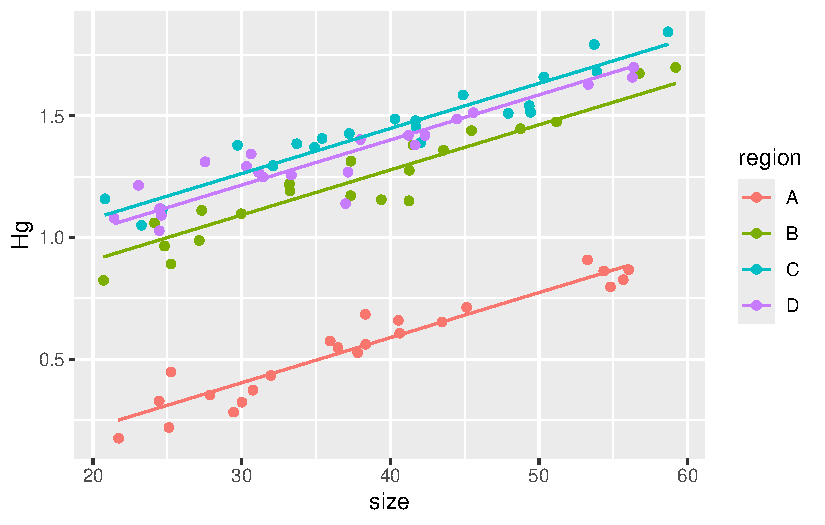
\includegraphics{mixed-effects_files/figure-pdf/unnamed-chunk-11-1.pdf}

\paragraph{How to obtain a population
``line''}\label{how-to-obtain-a-population-line}

\begin{Shaded}
\begin{Highlighting}[]
\NormalTok{preddata }\OtherTok{\textless{}{-}}\NormalTok{ HgDat\_df}
\NormalTok{preddata}\SpecialCharTok{$}\NormalTok{predHg }\OtherTok{\textless{}{-}} \FunctionTok{predict}\NormalTok{(m1, preddata)}
\NormalTok{preddata}\SpecialCharTok{$}\NormalTok{predHg\_population }\OtherTok{\textless{}{-}} \FunctionTok{predict}\NormalTok{(m1, preddata, }\AttributeTok{re.form=}\SpecialCharTok{\textasciitilde{}}\DecValTok{0}\NormalTok{)}

\FunctionTok{ggplot}\NormalTok{(}\AttributeTok{data=}\NormalTok{HgDat\_df, }\FunctionTok{aes}\NormalTok{(}\AttributeTok{x=}\NormalTok{size, }\AttributeTok{y=}\NormalTok{Hg, }\AttributeTok{col=}\NormalTok{region)) }\SpecialCharTok{+}
    \FunctionTok{geom\_point}\NormalTok{() }\SpecialCharTok{+}
    \FunctionTok{geom\_line}\NormalTok{(}\AttributeTok{data=}\NormalTok{preddata, }\FunctionTok{aes}\NormalTok{(}\AttributeTok{x=}\NormalTok{size, }\AttributeTok{y=}\NormalTok{predHg, }\AttributeTok{col=}\NormalTok{region))}\SpecialCharTok{+}
  \FunctionTok{geom\_line}\NormalTok{(}\AttributeTok{data=}\NormalTok{preddata, }\FunctionTok{aes}\NormalTok{(}\AttributeTok{x=}\NormalTok{size, }\AttributeTok{y=}\NormalTok{predHg\_population),                    }\AttributeTok{col=}\StringTok{\textquotesingle{}black\textquotesingle{}}\NormalTok{,}\AttributeTok{linewidth=}\FloatTok{1.5}\NormalTok{) }
\end{Highlighting}
\end{Shaded}

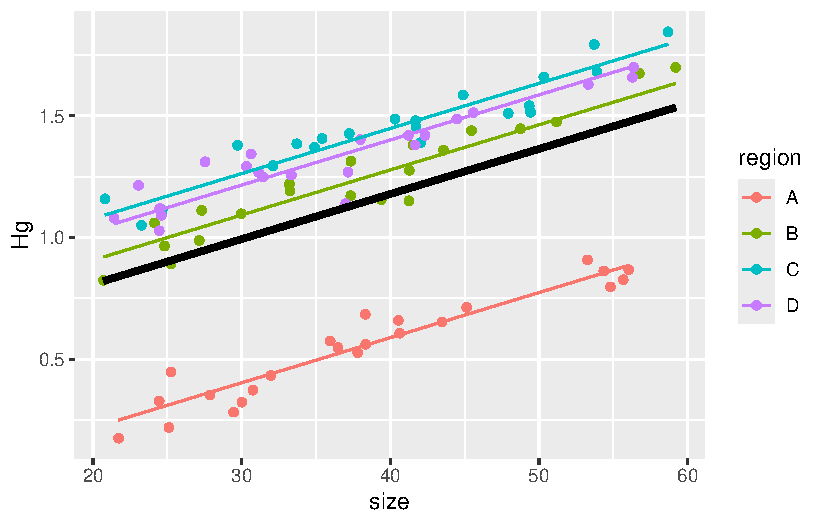
\includegraphics{mixed-effects_files/figure-pdf/unnamed-chunk-12-1.pdf}

Now, let's repeat this analysis, but in this case, let's assume the
intercept is fixed, and the slope is random

\begin{tcolorbox}[enhanced jigsaw, title=\textcolor{quarto-callout-important-color}{\faExclamation}\hspace{0.5em}{Question 1: points:10}, rightrule=.15mm, breakable, colbacktitle=quarto-callout-important-color!10!white, leftrule=.75mm, colback=white, bottomrule=.15mm, toprule=.15mm, opacitybacktitle=0.6, colframe=quarto-callout-important-color-frame, left=2mm, coltitle=black, opacityback=0, bottomtitle=1mm, toptitle=1mm, titlerule=0mm, arc=.35mm]

Simulate the same study, but in this case, there is a fixed intercept
and a random slope. 1) Present the equation you used for the simulation
(similar to the equation I showed in this document). 2) Run the
mixed-effects model, 3) Report whether the model output was a good
representation of reality, and 4) plot your model

\end{tcolorbox}

We have the model with fixed intercept and random slope

\[
Hg_{i,j} = 0.5+0.18(x_{i,j}+\psi_j) + \epsilon
\]\\

\begin{Shaded}
\begin{Highlighting}[]
\NormalTok{psi }\OtherTok{\textless{}{-}} \FunctionTok{rnorm}\NormalTok{(}\AttributeTok{n=}\DecValTok{4}\NormalTok{,}\AttributeTok{mean=}\DecValTok{0}\NormalTok{,}\AttributeTok{sd=}\FloatTok{0.25}\NormalTok{) }
\NormalTok{gamma }\OtherTok{\textless{}{-}} \DecValTok{0}
\NormalTok{N}\OtherTok{\textless{}{-}} \FunctionTok{round}\NormalTok{(}\FunctionTok{rnorm}\NormalTok{(}\DecValTok{4}\NormalTok{,}\DecValTok{20}\NormalTok{,}\DecValTok{2}\NormalTok{))}

\NormalTok{HgDat}\OtherTok{\textless{}{-}}\FunctionTok{list}\NormalTok{()}

\ControlFlowTok{for}\NormalTok{(i }\ControlFlowTok{in} \DecValTok{1}\SpecialCharTok{:}\DecValTok{4}\NormalTok{)\{}
\NormalTok{  x}\OtherTok{\textless{}{-}}\FunctionTok{runif}\NormalTok{(N[i],}\DecValTok{20}\NormalTok{,}\DecValTok{60}\NormalTok{)}
\NormalTok{  y}\OtherTok{\textless{}{-}}\FloatTok{0.5} \SpecialCharTok{+}\NormalTok{ (}\FloatTok{0.018}\SpecialCharTok{+}\NormalTok{psi[i])}\SpecialCharTok{*}\NormalTok{x }\SpecialCharTok{+}\NormalTok{ gamma }\SpecialCharTok{+} \FunctionTok{rnorm}\NormalTok{(N[i],}\DecValTok{0}\NormalTok{,}\FloatTok{0.08}\NormalTok{)}
\NormalTok{  Region}\OtherTok{\textless{}{-}}\FunctionTok{rep}\NormalTok{(LETTERS[i],N[i])}
\NormalTok{  HgDat[[i]]}\OtherTok{\textless{}{-}}\FunctionTok{data.frame}\NormalTok{(}\AttributeTok{size=}\NormalTok{x,}\AttributeTok{Hg=}\NormalTok{y,}\AttributeTok{region=}\NormalTok{Region)}
\NormalTok{\}}

\NormalTok{HgDat\_df}\OtherTok{\textless{}{-}}\FunctionTok{bind\_rows}\NormalTok{(HgDat)}
\NormalTok{HgDat\_df}\SpecialCharTok{$}\NormalTok{region}\OtherTok{\textless{}{-}}\FunctionTok{as.factor}\NormalTok{(HgDat\_df}\SpecialCharTok{$}\NormalTok{region)}

\FunctionTok{kbl}\NormalTok{(HgDat\_df, }\AttributeTok{col.names =} \FunctionTok{gsub}\NormalTok{(}\StringTok{"[.]"}\NormalTok{, }\StringTok{" "}\NormalTok{, }\FunctionTok{names}\NormalTok{(HgDat\_df)))}\SpecialCharTok{\%\textgreater{}\%}
  \FunctionTok{kable\_paper}\NormalTok{() }\SpecialCharTok{\%\textgreater{}\%}
  \FunctionTok{scroll\_box}\NormalTok{(}\AttributeTok{width =} \StringTok{"500px"}\NormalTok{, }\AttributeTok{height =} \StringTok{"200px"}\NormalTok{)}
\end{Highlighting}
\end{Shaded}

\begin{table}
\centering
\begin{tabular}[t]{r|r|l}
\hline
size & Hg & region\\
\hline
44.49633 & 3.7538735 & A\\
\hline
45.89681 & 3.9092576 & A\\
\hline
22.27424 & 2.1115534 & A\\
\hline
51.05273 & 4.0833499 & A\\
\hline
50.53021 & 4.0892541 & A\\
\hline
32.63227 & 2.8309382 & A\\
\hline
25.75203 & 2.2660819 & A\\
\hline
58.01478 & 4.7896050 & A\\
\hline
48.26798 & 3.9274908 & A\\
\hline
35.91883 & 3.0653145 & A\\
\hline
25.39562 & 2.4716503 & A\\
\hline
46.59767 & 3.8310754 & A\\
\hline
26.90454 & 2.5325610 & A\\
\hline
54.76171 & 4.5287399 & A\\
\hline
47.00335 & 3.9944346 & A\\
\hline
53.75383 & 4.4093597 & A\\
\hline
56.92890 & 4.6263921 & A\\
\hline
40.96317 & 3.4651435 & A\\
\hline
31.65698 & 2.6908401 & A\\
\hline
29.98829 & 2.7342171 & A\\
\hline
52.14664 & 4.2727786 & A\\
\hline
43.35757 & 3.6901237 & A\\
\hline
32.81201 & 0.9896216 & B\\
\hline
24.24138 & 0.7045335 & B\\
\hline
43.88285 & 0.8236133 & B\\
\hline
59.92679 & 0.9976705 & B\\
\hline
50.17995 & 0.9349966 & B\\
\hline
42.67223 & 1.0041640 & B\\
\hline
21.30427 & 0.7255842 & B\\
\hline
55.31300 & 1.0187260 & B\\
\hline
27.60575 & 0.8167307 & B\\
\hline
53.46462 & 0.8503216 & B\\
\hline
33.68350 & 0.7991693 & B\\
\hline
58.78693 & 1.1596891 & B\\
\hline
25.76395 & 0.7704838 & B\\
\hline
58.90586 & 0.9950072 & B\\
\hline
41.50829 & 0.8669849 & B\\
\hline
37.83168 & 0.9003682 & B\\
\hline
29.03923 & 0.6979645 & B\\
\hline
29.51890 & 7.5109493 & C\\
\hline
23.32747 & 5.9607912 & C\\
\hline
55.52368 & 13.5905191 & C\\
\hline
26.03121 & 6.6317937 & C\\
\hline
48.15941 & 11.9971759 & C\\
\hline
22.42474 & 5.7790031 & C\\
\hline
52.83746 & 13.1276758 & C\\
\hline
28.76440 & 7.3516638 & C\\
\hline
30.68447 & 7.8392250 & C\\
\hline
52.80883 & 12.9712524 & C\\
\hline
44.38067 & 10.9588245 & C\\
\hline
40.23206 & 10.0186583 & C\\
\hline
50.67936 & 12.5120190 & C\\
\hline
26.75878 & 6.8032520 & C\\
\hline
27.74998 & 7.1654581 & C\\
\hline
57.55533 & 14.3525601 & C\\
\hline
27.53701 & 7.0797740 & C\\
\hline
23.40895 & 5.7237214 & D\\
\hline
30.30715 & 7.3678787 & D\\
\hline
33.76864 & 7.9854485 & D\\
\hline
32.99386 & 7.7678953 & D\\
\hline
50.10875 & 11.6936969 & D\\
\hline
28.45669 & 7.0237824 & D\\
\hline
33.52164 & 7.8912770 & D\\
\hline
40.71390 & 9.4837654 & D\\
\hline
32.49876 & 7.7017561 & D\\
\hline
36.00520 & 8.4740572 & D\\
\hline
37.95420 & 8.8627601 & D\\
\hline
35.98533 & 8.4674989 & D\\
\hline
23.94258 & 5.8738819 & D\\
\hline
36.14803 & 8.4553560 & D\\
\hline
34.17900 & 8.1443605 & D\\
\hline
26.48389 & 6.3783979 & D\\
\hline
\end{tabular}
\end{table}

\begin{Shaded}
\begin{Highlighting}[]
\NormalTok{m2}\OtherTok{\textless{}{-}} \FunctionTok{glmmTMB}\NormalTok{(Hg}\SpecialCharTok{\textasciitilde{}}\NormalTok{size }\SpecialCharTok{+}\NormalTok{ (}\DecValTok{0}\SpecialCharTok{+}\NormalTok{size}\SpecialCharTok{|}\NormalTok{region), }\AttributeTok{data=}\NormalTok{HgDat\_df)}


\FunctionTok{summary}\NormalTok{(m2)}
\end{Highlighting}
\end{Shaded}

\begin{verbatim}
 Family: gaussian  ( identity )
Formula:          Hg ~ size + (0 + size | region)
Data: HgDat_df

     AIC      BIC   logLik deviance df.resid 
  -115.6   -106.5     61.8   -123.6       68 

Random effects:

Conditional model:
 Groups   Name Variance Std.Dev.
 region   size 0.009453 0.09723 
 Residual      0.005791 0.07610 
Number of obs: 72, groups:  region, 4

Dispersion estimate for gaussian family (sigma^2): 0.00579 

Conditional model:
            Estimate Std. Error z value Pr(>|z|)    
(Intercept)  0.51974    0.03362  15.460  < 2e-16 ***
size         0.13493    0.04862   2.775  0.00552 ** 
---
Signif. codes:  0 '***' 0.001 '**' 0.01 '*' 0.05 '.' 0.1 ' ' 1
\end{verbatim}

\begin{Shaded}
\begin{Highlighting}[]
\NormalTok{preddata }\OtherTok{\textless{}{-}}\NormalTok{ HgDat\_df}
\NormalTok{preddata}\SpecialCharTok{$}\NormalTok{predHg }\OtherTok{\textless{}{-}} \FunctionTok{predict}\NormalTok{(m2, preddata)}

\NormalTok{preddata }\OtherTok{\textless{}{-}}\NormalTok{ HgDat\_df}
\NormalTok{preddata}\SpecialCharTok{$}\NormalTok{predHg }\OtherTok{\textless{}{-}} \FunctionTok{predict}\NormalTok{(m2, preddata)}
\NormalTok{preddata}\SpecialCharTok{$}\NormalTok{predHg\_population }\OtherTok{\textless{}{-}} \FunctionTok{predict}\NormalTok{(m2, preddata, }\AttributeTok{re.form=}\SpecialCharTok{\textasciitilde{}}\DecValTok{0}\NormalTok{)}

\FunctionTok{ggplot}\NormalTok{(}\AttributeTok{data=}\NormalTok{HgDat\_df, }\FunctionTok{aes}\NormalTok{(}\AttributeTok{x=}\NormalTok{size, }\AttributeTok{y=}\NormalTok{Hg, }\AttributeTok{col=}\NormalTok{region)) }\SpecialCharTok{+}
    \FunctionTok{geom\_point}\NormalTok{() }\SpecialCharTok{+}
    \FunctionTok{geom\_line}\NormalTok{(}\AttributeTok{data=}\NormalTok{preddata, }\FunctionTok{aes}\NormalTok{(}\AttributeTok{x=}\NormalTok{size, }\AttributeTok{y=}\NormalTok{predHg, }\AttributeTok{col=}\NormalTok{region))}\SpecialCharTok{+}
  \FunctionTok{geom\_line}\NormalTok{(}\AttributeTok{data=}\NormalTok{preddata, }\FunctionTok{aes}\NormalTok{(}\AttributeTok{x=}\NormalTok{size, }\AttributeTok{y=}\NormalTok{predHg\_population),}\AttributeTok{col=}\StringTok{\textquotesingle{}black\textquotesingle{}}\NormalTok{,}\AttributeTok{linewidth=}\FloatTok{1.5}\NormalTok{) }
\end{Highlighting}
\end{Shaded}

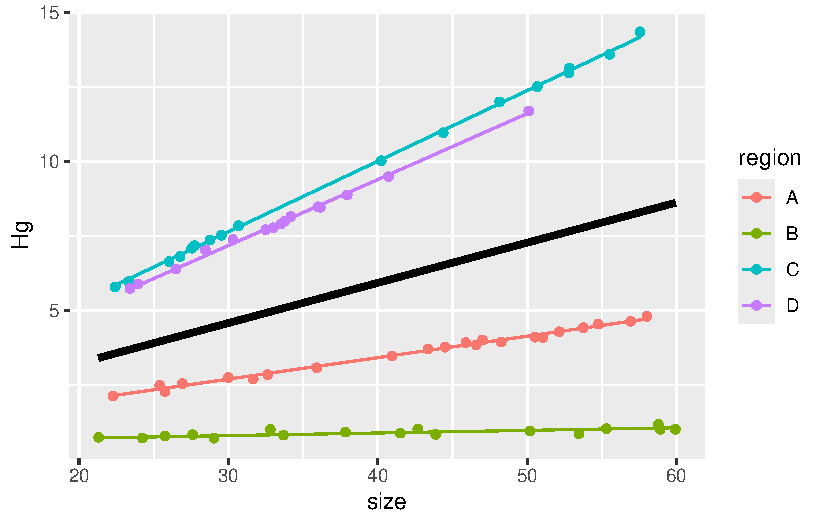
\includegraphics{mixed-effects_files/figure-pdf/unnamed-chunk-13-1.pdf}

\subsection{Answer 1.}\label{answer-1.}

\[
Hg_{i,j} = 0.5+0.18(x_{i,j}+\psi_j) + \epsilon
\]

The p-value for the fixed intercept is significant, but the p-value for
the random slope is \(0.459>0.05\), which is not significant. Thus, this
model may not be the best fit.

\begin{tcolorbox}[enhanced jigsaw, title=\textcolor{quarto-callout-important-color}{\faExclamation}\hspace{0.5em}{Question 2. Points: 10}, rightrule=.15mm, breakable, colbacktitle=quarto-callout-important-color!10!white, leftrule=.75mm, colback=white, bottomrule=.15mm, toprule=.15mm, opacitybacktitle=0.6, colframe=quarto-callout-important-color-frame, left=2mm, coltitle=black, opacityback=0, bottomtitle=1mm, toptitle=1mm, titlerule=0mm, arc=.35mm]

Simulate the same study, but in this case, there is a random intercept
and a random slope. 1) Present the equation you used for the simulation
(similar to the equation I showed in this document). 2) Run the
mixed-effects model, 3) Report whether the model output was a good
representation of reality, and 4) plot your model

\end{tcolorbox}

\begin{Shaded}
\begin{Highlighting}[]
\NormalTok{psi }\OtherTok{\textless{}{-}} \FunctionTok{rnorm}\NormalTok{(}\AttributeTok{n=}\DecValTok{4}\NormalTok{,}\AttributeTok{mean=}\DecValTok{0}\NormalTok{,}\AttributeTok{sd=}\FloatTok{0.25}\NormalTok{) }
\NormalTok{gamma }\OtherTok{\textless{}{-}} \FunctionTok{rnorm}\NormalTok{(}\AttributeTok{n=}\DecValTok{4}\NormalTok{,}\AttributeTok{mean=}\DecValTok{0}\NormalTok{,}\AttributeTok{sd=}\FloatTok{0.25}\NormalTok{) }
\NormalTok{N}\OtherTok{\textless{}{-}} \FunctionTok{round}\NormalTok{(}\FunctionTok{rnorm}\NormalTok{(}\DecValTok{4}\NormalTok{,}\DecValTok{20}\NormalTok{,}\DecValTok{2}\NormalTok{))}

\NormalTok{HgDat}\OtherTok{\textless{}{-}}\FunctionTok{list}\NormalTok{()}


\ControlFlowTok{for}\NormalTok{(i }\ControlFlowTok{in} \DecValTok{1}\SpecialCharTok{:}\DecValTok{4}\NormalTok{)\{}
\NormalTok{  x}\OtherTok{\textless{}{-}}\FunctionTok{runif}\NormalTok{(N[i],}\DecValTok{20}\NormalTok{,}\DecValTok{60}\NormalTok{)}
\NormalTok{  y}\OtherTok{\textless{}{-}}\FloatTok{0.5} \SpecialCharTok{+}\NormalTok{ (}\FloatTok{0.018}\SpecialCharTok{+}\NormalTok{psi[i])}\SpecialCharTok{*}\NormalTok{x }\SpecialCharTok{+}\NormalTok{ gamma[i] }\SpecialCharTok{+} \FunctionTok{rnorm}\NormalTok{(N[i],}\DecValTok{0}\NormalTok{,}\FloatTok{0.08}\NormalTok{)}
\NormalTok{  Region}\OtherTok{\textless{}{-}}\FunctionTok{rep}\NormalTok{(LETTERS[i],N[i])}
\NormalTok{  HgDat[[i]]}\OtherTok{\textless{}{-}}\FunctionTok{data.frame}\NormalTok{(}\AttributeTok{size=}\NormalTok{x,}\AttributeTok{Hg=}\NormalTok{y,}\AttributeTok{region=}\NormalTok{Region)}
\NormalTok{\}}

\NormalTok{HgDat\_df}\OtherTok{\textless{}{-}}\FunctionTok{bind\_rows}\NormalTok{(HgDat)}
\NormalTok{HgDat\_df}\SpecialCharTok{$}\NormalTok{region}\OtherTok{\textless{}{-}}\FunctionTok{as.factor}\NormalTok{(HgDat\_df}\SpecialCharTok{$}\NormalTok{region)}

\FunctionTok{kbl}\NormalTok{(HgDat\_df, }\AttributeTok{col.names =} \FunctionTok{gsub}\NormalTok{(}\StringTok{"[.]"}\NormalTok{, }\StringTok{" "}\NormalTok{, }\FunctionTok{names}\NormalTok{(HgDat\_df)))}\SpecialCharTok{\%\textgreater{}\%}
  \FunctionTok{kable\_paper}\NormalTok{() }\SpecialCharTok{\%\textgreater{}\%}
  \FunctionTok{scroll\_box}\NormalTok{(}\AttributeTok{width =} \StringTok{"500px"}\NormalTok{, }\AttributeTok{height =} \StringTok{"200px"}\NormalTok{)}
\end{Highlighting}
\end{Shaded}

\begin{table}
\centering
\begin{tabular}[t]{r|r|l}
\hline
size & Hg & region\\
\hline
31.40879 & -0.5988094 & A\\
\hline
34.08152 & -0.6945361 & A\\
\hline
54.51222 & -1.4915502 & A\\
\hline
49.34688 & -1.4271821 & A\\
\hline
54.93623 & -1.6455704 & A\\
\hline
24.22206 & -0.3110356 & A\\
\hline
22.81448 & -0.3066756 & A\\
\hline
58.31181 & -1.7928674 & A\\
\hline
44.33808 & -1.1163633 & A\\
\hline
55.74338 & -1.6076756 & A\\
\hline
59.21084 & -1.6929282 & A\\
\hline
27.40456 & -0.6057446 & A\\
\hline
53.04921 & -1.4831494 & A\\
\hline
35.11276 & -0.8123434 & A\\
\hline
31.33799 & -0.6376926 & A\\
\hline
31.91727 & -0.6652387 & A\\
\hline
56.77740 & -1.5672870 & A\\
\hline
59.70154 & -1.9015779 & A\\
\hline
57.03275 & -1.7135137 & A\\
\hline
41.00744 & -0.9318195 & A\\
\hline
31.02216 & -0.5464400 & A\\
\hline
31.71038 & -0.6448614 & A\\
\hline
24.41385 & 3.9370734 & B\\
\hline
40.44125 & 6.0443147 & B\\
\hline
59.94030 & 8.7244708 & B\\
\hline
38.13316 & 5.7103045 & B\\
\hline
43.08266 & 6.4791922 & B\\
\hline
51.16490 & 7.3963668 & B\\
\hline
33.85497 & 5.3115754 & B\\
\hline
40.89564 & 6.0180471 & B\\
\hline
58.46399 & 8.5165351 & B\\
\hline
25.60348 & 4.0462132 & B\\
\hline
32.16446 & 5.0147764 & B\\
\hline
33.61851 & 5.2080602 & B\\
\hline
56.24478 & 8.2763082 & B\\
\hline
34.28227 & 5.3034947 & B\\
\hline
39.80641 & 6.0226082 & B\\
\hline
55.22005 & 8.0596844 & B\\
\hline
48.62708 & 7.2526882 & B\\
\hline
39.23195 & 5.9297849 & B\\
\hline
20.57770 & 3.2975116 & B\\
\hline
23.78686 & 3.9350198 & B\\
\hline
57.72715 & 19.8413765 & C\\
\hline
44.89145 & 15.5436539 & C\\
\hline
38.89602 & 13.4732139 & C\\
\hline
30.76753 & 10.8383693 & C\\
\hline
35.41723 & 12.2139599 & C\\
\hline
58.75629 & 20.3282924 & C\\
\hline
23.08377 & 8.3238306 & C\\
\hline
26.06057 & 9.3539705 & C\\
\hline
31.35674 & 10.9995154 & C\\
\hline
35.67728 & 12.6812085 & C\\
\hline
34.64976 & 12.3055658 & C\\
\hline
58.65066 & 20.4304983 & C\\
\hline
32.13051 & 11.3901655 & C\\
\hline
59.55810 & 20.5544667 & C\\
\hline
38.18007 & 13.3472469 & C\\
\hline
47.35179 & 16.3872034 & C\\
\hline
26.32638 & 9.3262287 & C\\
\hline
53.67211 & 18.6116249 & C\\
\hline
53.47945 & 18.3913552 & C\\
\hline
35.32127 & 0.1063369 & D\\
\hline
58.57851 & 0.1384798 & D\\
\hline
46.79525 & 0.0921137 & D\\
\hline
51.38501 & 0.0882791 & D\\
\hline
43.26929 & 0.0714167 & D\\
\hline
29.04651 & 0.0754621 & D\\
\hline
42.84702 & -0.0232572 & D\\
\hline
48.17618 & 0.0193926 & D\\
\hline
21.31261 & 0.2128523 & D\\
\hline
53.62898 & 0.0418465 & D\\
\hline
39.18316 & -0.0938177 & D\\
\hline
47.51750 & 0.0411739 & D\\
\hline
46.87465 & 0.1110700 & D\\
\hline
57.87244 & 0.0237888 & D\\
\hline
46.09601 & 0.1143560 & D\\
\hline
27.45446 & 0.2319380 & D\\
\hline
47.09357 & 0.1979479 & D\\
\hline
\end{tabular}
\end{table}

\begin{Shaded}
\begin{Highlighting}[]
\NormalTok{m3}\OtherTok{\textless{}{-}} \FunctionTok{glmmTMB}\NormalTok{(Hg}\SpecialCharTok{\textasciitilde{}}\NormalTok{size }\SpecialCharTok{+}\NormalTok{ (}\DecValTok{1} \SpecialCharTok{+}\NormalTok{ size}\SpecialCharTok{|}\NormalTok{region), }\AttributeTok{data=}\NormalTok{HgDat\_df)}

\FunctionTok{summary}\NormalTok{(m3)}
\end{Highlighting}
\end{Shaded}

\begin{verbatim}
 Family: gaussian  ( identity )
Formula:          Hg ~ size + (1 + size | region)
Data: HgDat_df

     AIC      BIC   logLik deviance df.resid 
  -102.4    -88.2     57.2   -114.4       72 

Random effects:

Conditional model:
 Groups   Name        Variance Std.Dev. Corr 
 region   (Intercept) 0.02418  0.15549       
          size        0.02185  0.14782  0.15 
 Residual             0.00678  0.08234       
Number of obs: 78, groups:  region, 4

Dispersion estimate for gaussian family (sigma^2): 0.00678 

Conditional model:
            Estimate Std. Error z value Pr(>|z|)    
(Intercept)  0.51082    0.08576   5.956 2.58e-09 ***
size         0.10670    0.07392   1.444    0.149    
---
Signif. codes:  0 '***' 0.001 '**' 0.01 '*' 0.05 '.' 0.1 ' ' 1
\end{verbatim}

\begin{Shaded}
\begin{Highlighting}[]
\NormalTok{preddata }\OtherTok{\textless{}{-}}\NormalTok{ HgDat\_df}
\NormalTok{preddata}\SpecialCharTok{$}\NormalTok{predHg }\OtherTok{\textless{}{-}} \FunctionTok{predict}\NormalTok{(m3, preddata)}
\NormalTok{preddata}\SpecialCharTok{$}\NormalTok{predHg\_population }\OtherTok{\textless{}{-}} \FunctionTok{predict}\NormalTok{(m3, preddata, }\AttributeTok{re.form=}\SpecialCharTok{\textasciitilde{}}\DecValTok{0}\NormalTok{)}

\FunctionTok{ggplot}\NormalTok{(}\AttributeTok{data=}\NormalTok{HgDat\_df, }\FunctionTok{aes}\NormalTok{(}\AttributeTok{x=}\NormalTok{size, }\AttributeTok{y=}\NormalTok{Hg, }\AttributeTok{col=}\NormalTok{region)) }\SpecialCharTok{+}
    \FunctionTok{geom\_point}\NormalTok{() }\SpecialCharTok{+}
    \FunctionTok{geom\_line}\NormalTok{(}\AttributeTok{data=}\NormalTok{preddata, }\FunctionTok{aes}\NormalTok{(}\AttributeTok{x=}\NormalTok{size, }\AttributeTok{y=}\NormalTok{predHg, }\AttributeTok{col=}\NormalTok{region))}\SpecialCharTok{+}
  \FunctionTok{geom\_line}\NormalTok{(}\AttributeTok{data=}\NormalTok{preddata, }\FunctionTok{aes}\NormalTok{(}\AttributeTok{x=}\NormalTok{size, }\AttributeTok{y=}\NormalTok{predHg\_population),                    }\AttributeTok{col=}\StringTok{\textquotesingle{}black\textquotesingle{}}\NormalTok{,}\AttributeTok{linewidth=}\FloatTok{1.5}\NormalTok{) }
\end{Highlighting}
\end{Shaded}

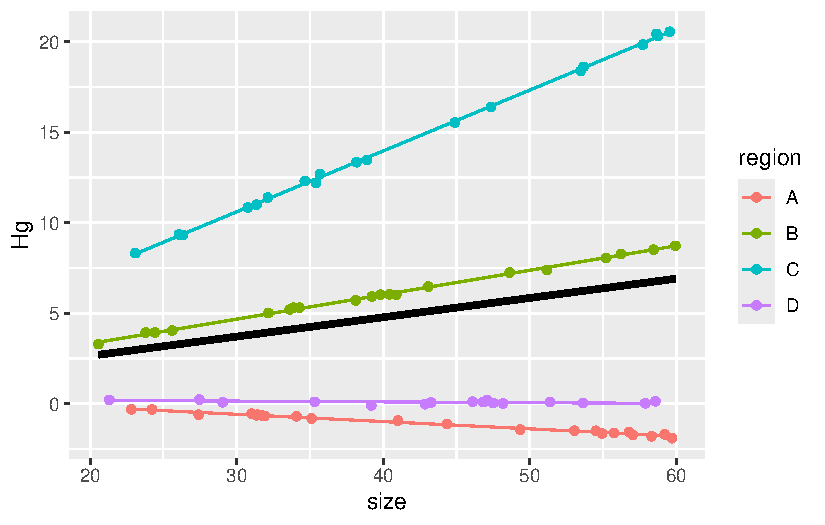
\includegraphics{mixed-effects_files/figure-pdf/unnamed-chunk-14-1.pdf}

\subsection{Answer 2}\label{answer-2}

\[
Hg_{i,j} = 0.5+0.18(x_{i,j}+\psi_j) + \gamma_j + \epsilon
\] The p-value for the fixed intercept is significant, but the p-value
for the random slope is \(0.872>0.05\), which is not significant. Thus,
this model may not be the best fit.

Finally, let's look at what happens with a low N.

You will repeat question 2, but using the following to obtain your
sample:

\subsection{Question 3}\label{question-3}

\begin{Shaded}
\begin{Highlighting}[]
\NormalTok{psi }\OtherTok{\textless{}{-}} \FunctionTok{rnorm}\NormalTok{(}\AttributeTok{n=}\DecValTok{4}\NormalTok{,}\AttributeTok{mean=}\DecValTok{0}\NormalTok{,}\AttributeTok{sd=}\FloatTok{0.25}\NormalTok{) }
\NormalTok{gamma }\OtherTok{\textless{}{-}} \FunctionTok{rnorm}\NormalTok{(}\AttributeTok{n=}\DecValTok{4}\NormalTok{,}\AttributeTok{mean=}\DecValTok{0}\NormalTok{,}\AttributeTok{sd=}\FloatTok{0.25}\NormalTok{)}
\NormalTok{N}\OtherTok{\textless{}{-}} \FunctionTok{round}\NormalTok{(}\FunctionTok{rnorm}\NormalTok{(}\DecValTok{4}\NormalTok{,}\DecValTok{150}\NormalTok{,}\DecValTok{20}\NormalTok{))}

\NormalTok{HgDat}\OtherTok{\textless{}{-}}\FunctionTok{list}\NormalTok{()}


\ControlFlowTok{for}\NormalTok{(i }\ControlFlowTok{in} \DecValTok{1}\SpecialCharTok{:}\DecValTok{4}\NormalTok{)\{}
\NormalTok{  x}\OtherTok{\textless{}{-}}\FunctionTok{runif}\NormalTok{(N[i],}\DecValTok{20}\NormalTok{,}\DecValTok{60}\NormalTok{)}
\NormalTok{  y}\OtherTok{\textless{}{-}}\FloatTok{0.5} \SpecialCharTok{+}\NormalTok{ (}\FloatTok{0.018}\SpecialCharTok{+}\NormalTok{psi[i])}\SpecialCharTok{*}\NormalTok{x }\SpecialCharTok{+}\NormalTok{ gamma[i] }\SpecialCharTok{+} \FunctionTok{rnorm}\NormalTok{(N[i],}\DecValTok{0}\NormalTok{,}\FloatTok{0.08}\NormalTok{)}
\NormalTok{  Region}\OtherTok{\textless{}{-}}\FunctionTok{rep}\NormalTok{(LETTERS[i],N[i])}
\NormalTok{  HgDat[[i]]}\OtherTok{\textless{}{-}}\FunctionTok{data.frame}\NormalTok{(}\AttributeTok{size=}\NormalTok{x,}\AttributeTok{Hg=}\NormalTok{y,}\AttributeTok{region=}\NormalTok{Region)}
\NormalTok{\}}

\NormalTok{HgDat\_df}\OtherTok{\textless{}{-}}\FunctionTok{bind\_rows}\NormalTok{(HgDat)}
\NormalTok{HgDat\_df}\SpecialCharTok{$}\NormalTok{region}\OtherTok{\textless{}{-}}\FunctionTok{as.factor}\NormalTok{(HgDat\_df}\SpecialCharTok{$}\NormalTok{region)}

\FunctionTok{kbl}\NormalTok{(HgDat\_df, }\AttributeTok{col.names =} \FunctionTok{gsub}\NormalTok{(}\StringTok{"[.]"}\NormalTok{, }\StringTok{" "}\NormalTok{, }\FunctionTok{names}\NormalTok{(HgDat\_df)))}\SpecialCharTok{\%\textgreater{}\%}
  \FunctionTok{kable\_paper}\NormalTok{() }\SpecialCharTok{\%\textgreater{}\%}
  \FunctionTok{scroll\_box}\NormalTok{(}\AttributeTok{width =} \StringTok{"500px"}\NormalTok{, }\AttributeTok{height =} \StringTok{"200px"}\NormalTok{)}
\end{Highlighting}
\end{Shaded}

\begin{table}
\centering
\begin{tabular}[t]{r|r|l}
\hline
size & Hg & region\\
\hline
47.03911 & 13.261229 & A\\
\hline
42.91721 & 11.845123 & A\\
\hline
29.62873 & 8.160534 & A\\
\hline
33.92795 & 9.566759 & A\\
\hline
52.29348 & 14.363485 & A\\
\hline
50.33929 & 13.972527 & A\\
\hline
53.69048 & 14.790631 & A\\
\hline
58.22425 & 16.119977 & A\\
\hline
41.17877 & 11.467922 & A\\
\hline
48.09510 & 13.280486 & A\\
\hline
55.91142 & 15.327752 & A\\
\hline
32.38006 & 9.081811 & A\\
\hline
27.26504 & 7.739584 & A\\
\hline
25.00352 & 7.034259 & A\\
\hline
24.19327 & 6.886057 & A\\
\hline
56.00084 & 15.391384 & A\\
\hline
49.98570 & 13.807229 & A\\
\hline
21.10812 & 6.097785 & A\\
\hline
22.00870 & 6.326785 & A\\
\hline
29.47896 & 8.287703 & A\\
\hline
34.82179 & 9.732903 & A\\
\hline
34.01623 & 9.511499 & A\\
\hline
22.81249 & 6.554907 & A\\
\hline
54.33663 & 14.936435 & A\\
\hline
36.07548 & 9.968535 & A\\
\hline
31.05927 & 8.650916 & A\\
\hline
28.32302 & 8.032601 & A\\
\hline
36.84292 & 10.367155 & A\\
\hline
24.56583 & 7.029963 & A\\
\hline
32.38412 & 9.070681 & A\\
\hline
25.56707 & 7.107475 & A\\
\hline
57.88682 & 16.012726 & A\\
\hline
48.81995 & 13.435786 & A\\
\hline
23.67716 & 6.611977 & A\\
\hline
42.10429 & 11.647280 & A\\
\hline
22.30010 & 6.400589 & A\\
\hline
37.70970 & 10.507509 & A\\
\hline
43.14648 & 12.087111 & A\\
\hline
51.65307 & 14.303108 & A\\
\hline
33.18967 & 9.217342 & A\\
\hline
48.83311 & 13.519972 & A\\
\hline
49.06692 & 13.576659 & A\\
\hline
25.99555 & 7.263181 & A\\
\hline
34.31131 & 9.596301 & A\\
\hline
33.91408 & 9.401638 & A\\
\hline
33.12783 & 9.300960 & A\\
\hline
42.82193 & 11.839422 & A\\
\hline
44.47295 & 12.203027 & A\\
\hline
56.98992 & 15.647985 & A\\
\hline
39.17379 & 10.981375 & A\\
\hline
55.88068 & 15.433538 & A\\
\hline
30.07538 & 8.662103 & A\\
\hline
34.28996 & 9.699090 & A\\
\hline
58.19083 & 15.879564 & A\\
\hline
23.62509 & 6.605349 & A\\
\hline
40.70638 & 11.358375 & A\\
\hline
24.71946 & 7.146322 & A\\
\hline
50.67316 & 13.938896 & A\\
\hline
27.52590 & 7.854441 & A\\
\hline
23.12418 & 6.604248 & A\\
\hline
30.60156 & 8.604117 & A\\
\hline
47.95802 & 13.333376 & A\\
\hline
39.25008 & 10.917178 & A\\
\hline
51.75690 & 14.206660 & A\\
\hline
40.12740 & 11.124925 & A\\
\hline
53.88196 & 14.841725 & A\\
\hline
57.47734 & 15.875109 & A\\
\hline
56.87089 & 15.628226 & A\\
\hline
32.43425 & 9.180408 & A\\
\hline
51.56324 & 14.328182 & A\\
\hline
21.35995 & 6.165795 & A\\
\hline
24.44268 & 7.067890 & A\\
\hline
40.30130 & 11.138157 & A\\
\hline
40.91863 & 11.354504 & A\\
\hline
43.00460 & 11.944969 & A\\
\hline
56.60961 & 15.575314 & A\\
\hline
40.76895 & 11.476526 & A\\
\hline
54.49856 & 15.098099 & A\\
\hline
43.44780 & 11.957207 & A\\
\hline
37.06362 & 10.207187 & A\\
\hline
38.88630 & 10.718106 & A\\
\hline
43.06665 & 12.139178 & A\\
\hline
23.89601 & 6.806851 & A\\
\hline
24.03497 & 6.778091 & A\\
\hline
44.98719 & 12.395874 & A\\
\hline
55.21401 & 15.204098 & A\\
\hline
26.75089 & 7.553331 & A\\
\hline
26.64081 & 7.558144 & A\\
\hline
30.84041 & 8.773444 & A\\
\hline
35.50108 & 9.916031 & A\\
\hline
57.03745 & 15.630983 & A\\
\hline
34.91685 & 9.763054 & A\\
\hline
25.51567 & 7.126933 & A\\
\hline
53.02406 & 14.648140 & A\\
\hline
27.88486 & 7.872027 & A\\
\hline
42.10524 & 11.776910 & A\\
\hline
57.35509 & 15.829198 & A\\
\hline
54.59907 & 15.098898 & A\\
\hline
23.40085 & 6.612932 & A\\
\hline
23.80477 & 6.821042 & A\\
\hline
22.00354 & 6.370126 & A\\
\hline
57.92781 & 15.865659 & A\\
\hline
45.25947 & 12.578243 & A\\
\hline
31.47696 & 8.815186 & A\\
\hline
22.79239 & 6.577708 & A\\
\hline
33.95440 & 9.504883 & A\\
\hline
43.09490 & 12.198247 & A\\
\hline
22.00766 & 6.254959 & A\\
\hline
24.95862 & 7.140377 & A\\
\hline
40.04180 & 11.119670 & A\\
\hline
49.42673 & 13.527468 & A\\
\hline
20.13424 & 5.805466 & A\\
\hline
37.34719 & 10.372604 & A\\
\hline
39.11074 & 10.891618 & A\\
\hline
24.04245 & 6.980753 & A\\
\hline
40.94615 & 11.334829 & A\\
\hline
34.18971 & 9.535508 & A\\
\hline
47.01937 & 12.847221 & A\\
\hline
44.84563 & 12.350830 & A\\
\hline
55.42971 & 15.391576 & A\\
\hline
42.27968 & 11.632485 & A\\
\hline
31.87466 & 8.865345 & A\\
\hline
54.59276 & 15.113677 & A\\
\hline
59.51880 & 16.431809 & A\\
\hline
28.69769 & 8.198092 & A\\
\hline
29.23953 & 8.363290 & A\\
\hline
42.73135 & 11.855513 & A\\
\hline
45.63744 & 12.541897 & A\\
\hline
55.22039 & 15.169721 & A\\
\hline
25.27385 & 7.218863 & A\\
\hline
41.76172 & 11.500882 & A\\
\hline
42.04254 & 11.642964 & A\\
\hline
42.46182 & 11.908883 & A\\
\hline
46.71418 & 12.913009 & A\\
\hline
33.86300 & 9.421131 & A\\
\hline
38.58188 & 10.657150 & A\\
\hline
57.79327 & 15.905674 & A\\
\hline
37.93770 & 10.448003 & A\\
\hline
31.87606 & 9.020912 & A\\
\hline
32.97749 & 9.281504 & A\\
\hline
34.09926 & 9.638168 & A\\
\hline
28.80303 & 8.032073 & A\\
\hline
34.82286 & 9.798923 & A\\
\hline
30.73599 & 8.602005 & A\\
\hline
29.90515 & 8.301881 & A\\
\hline
26.80996 & 7.611438 & A\\
\hline
44.11448 & 12.237027 & A\\
\hline
29.33713 & 8.309267 & A\\
\hline
34.86957 & 9.709018 & A\\
\hline
32.31618 & 9.046519 & A\\
\hline
26.91445 & 7.450871 & A\\
\hline
48.05819 & 13.284740 & A\\
\hline
57.19256 & 15.827126 & A\\
\hline
26.84643 & 7.700545 & A\\
\hline
35.12616 & 9.956369 & A\\
\hline
42.27236 & 11.661141 & A\\
\hline
24.35789 & 7.048356 & A\\
\hline
30.02606 & 8.476851 & A\\
\hline
34.88382 & 9.733521 & A\\
\hline
38.06165 & 10.521524 & A\\
\hline
42.44226 & 11.658438 & A\\
\hline
24.97864 & 7.423461 & A\\
\hline
31.79124 & 8.900088 & A\\
\hline
41.21814 & 11.774014 & B\\
\hline
30.62884 & 8.979159 & B\\
\hline
42.40481 & 12.064699 & B\\
\hline
30.19860 & 8.927888 & B\\
\hline
54.66804 & 15.502534 & B\\
\hline
56.50041 & 15.987466 & B\\
\hline
29.49046 & 8.761238 & B\\
\hline
33.60593 & 9.846125 & B\\
\hline
47.71711 & 13.703710 & B\\
\hline
43.18709 & 12.364727 & B\\
\hline
39.37727 & 11.343772 & B\\
\hline
55.06748 & 15.623250 & B\\
\hline
46.82956 & 13.369442 & B\\
\hline
53.37502 & 15.140798 & B\\
\hline
27.63227 & 8.211684 & B\\
\hline
22.80777 & 6.883607 & B\\
\hline
42.56697 & 12.379532 & B\\
\hline
46.17414 & 13.267412 & B\\
\hline
40.78616 & 11.777299 & B\\
\hline
38.45508 & 11.070747 & B\\
\hline
54.49674 & 15.445771 & B\\
\hline
58.38699 & 16.444416 & B\\
\hline
32.73435 & 9.532685 & B\\
\hline
59.37299 & 16.809723 & B\\
\hline
53.16690 & 15.145898 & B\\
\hline
29.51574 & 8.774001 & B\\
\hline
34.31550 & 9.907820 & B\\
\hline
22.84590 & 6.977193 & B\\
\hline
48.66843 & 13.943769 & B\\
\hline
30.96356 & 9.168470 & B\\
\hline
58.31241 & 16.483932 & B\\
\hline
50.49479 & 14.209615 & B\\
\hline
33.94155 & 9.995230 & B\\
\hline
44.44294 & 12.892009 & B\\
\hline
38.83921 & 11.338773 & B\\
\hline
30.60767 & 8.857302 & B\\
\hline
46.85512 & 13.437910 & B\\
\hline
41.50780 & 12.005375 & B\\
\hline
41.19351 & 11.869376 & B\\
\hline
47.10385 & 13.358139 & B\\
\hline
39.68298 & 11.405969 & B\\
\hline
52.80681 & 15.007291 & B\\
\hline
53.86442 & 15.273271 & B\\
\hline
56.98082 & 16.236653 & B\\
\hline
31.00017 & 9.205170 & B\\
\hline
21.29851 & 6.555307 & B\\
\hline
58.14852 & 16.340872 & B\\
\hline
44.26162 & 12.740757 & B\\
\hline
40.60621 & 11.641619 & B\\
\hline
59.05409 & 16.678886 & B\\
\hline
38.93969 & 11.124681 & B\\
\hline
55.86576 & 15.946072 & B\\
\hline
44.26133 & 12.605775 & B\\
\hline
45.35069 & 12.951131 & B\\
\hline
51.71664 & 14.714002 & B\\
\hline
22.11716 & 6.598549 & B\\
\hline
22.64932 & 6.664698 & B\\
\hline
49.54430 & 14.112829 & B\\
\hline
45.97788 & 13.151513 & B\\
\hline
57.18691 & 16.141400 & B\\
\hline
24.96196 & 7.408534 & B\\
\hline
24.98046 & 7.392111 & B\\
\hline
59.94839 & 16.921817 & B\\
\hline
28.34398 & 8.259642 & B\\
\hline
23.44976 & 7.171540 & B\\
\hline
50.53520 & 14.369855 & B\\
\hline
56.13317 & 15.809432 & B\\
\hline
46.93562 & 13.544547 & B\\
\hline
49.35229 & 14.098295 & B\\
\hline
21.54336 & 6.698054 & B\\
\hline
41.90921 & 11.915271 & B\\
\hline
29.23933 & 8.610081 & B\\
\hline
52.07897 & 14.839911 & B\\
\hline
24.95594 & 7.330927 & B\\
\hline
28.13613 & 8.340965 & B\\
\hline
46.24449 & 13.244529 & B\\
\hline
35.23914 & 10.360944 & B\\
\hline
35.24239 & 10.322629 & B\\
\hline
37.64613 & 10.684725 & B\\
\hline
51.92608 & 14.823402 & B\\
\hline
53.16128 & 15.061836 & B\\
\hline
34.65083 & 10.113106 & B\\
\hline
36.64500 & 10.539243 & B\\
\hline
54.94057 & 15.587941 & B\\
\hline
27.46487 & 8.221046 & B\\
\hline
33.06413 & 9.623463 & B\\
\hline
41.39763 & 11.876418 & B\\
\hline
26.21048 & 7.851606 & B\\
\hline
38.66584 & 11.336393 & B\\
\hline
57.89700 & 16.405212 & B\\
\hline
29.52240 & 8.607009 & B\\
\hline
48.95411 & 13.943381 & B\\
\hline
56.38938 & 15.939854 & B\\
\hline
40.20883 & 11.612908 & B\\
\hline
25.45087 & 7.626195 & B\\
\hline
22.80668 & 6.906845 & B\\
\hline
51.72565 & 14.798507 & B\\
\hline
37.95717 & 10.952443 & B\\
\hline
29.17089 & 8.743153 & B\\
\hline
28.32128 & 8.541664 & B\\
\hline
47.30401 & 13.430115 & B\\
\hline
21.47964 & 6.421747 & B\\
\hline
58.23317 & 16.393215 & B\\
\hline
59.55860 & 16.822976 & B\\
\hline
33.50016 & 9.810119 & B\\
\hline
31.39440 & 9.159519 & B\\
\hline
36.63418 & 10.439268 & B\\
\hline
54.21306 & 15.566963 & B\\
\hline
23.70416 & 7.229260 & B\\
\hline
40.87002 & 11.812073 & B\\
\hline
43.26671 & 12.388235 & B\\
\hline
29.06339 & 8.610871 & B\\
\hline
49.00661 & 13.898973 & B\\
\hline
50.71757 & 14.427356 & B\\
\hline
54.62276 & 15.517864 & B\\
\hline
50.01668 & 14.310847 & B\\
\hline
23.98567 & 7.185940 & B\\
\hline
37.88875 & 10.980741 & B\\
\hline
54.62141 & 15.487878 & B\\
\hline
51.65809 & 14.557298 & B\\
\hline
29.10264 & 8.672496 & B\\
\hline
52.49938 & 14.963068 & B\\
\hline
47.73025 & 13.580180 & B\\
\hline
29.84448 & 8.811023 & B\\
\hline
38.61359 & 10.930894 & B\\
\hline
55.82059 & 15.816044 & B\\
\hline
22.97677 & 6.929409 & B\\
\hline
35.86035 & 10.314471 & B\\
\hline
41.96553 & 12.153583 & B\\
\hline
53.83779 & 15.336606 & B\\
\hline
34.43321 & 10.022972 & B\\
\hline
36.85479 & 10.688335 & B\\
\hline
51.51402 & 14.660917 & B\\
\hline
44.88339 & 13.009706 & B\\
\hline
32.89889 & 9.490613 & B\\
\hline
37.03761 & 10.712036 & B\\
\hline
39.74889 & 11.426882 & B\\
\hline
30.07922 & 8.865446 & B\\
\hline
47.44868 & 13.685717 & B\\
\hline
56.25340 & 15.785078 & B\\
\hline
31.73657 & 9.304393 & B\\
\hline
36.96857 & 10.747703 & B\\
\hline
48.93012 & 13.918436 & B\\
\hline
40.10601 & 11.643112 & B\\
\hline
32.11525 & 9.364913 & B\\
\hline
25.07270 & 7.441126 & B\\
\hline
54.57460 & 15.342129 & B\\
\hline
34.28651 & 10.013454 & B\\
\hline
24.43543 & 7.208620 & B\\
\hline
36.48351 & 10.584122 & B\\
\hline
30.17773 & 8.750646 & B\\
\hline
39.25202 & 11.437088 & B\\
\hline
42.56375 & 12.168564 & B\\
\hline
34.08540 & 9.924564 & B\\
\hline
38.54568 & 11.201567 & B\\
\hline
38.26646 & 11.047193 & B\\
\hline
32.04269 & 9.336641 & B\\
\hline
49.94715 & 14.235229 & B\\
\hline
44.68713 & 12.756950 & B\\
\hline
39.16804 & 11.244900 & B\\
\hline
36.85791 & 10.677115 & B\\
\hline
30.01509 & 8.749372 & B\\
\hline
20.72279 & 6.167039 & B\\
\hline
20.24008 & 6.123528 & B\\
\hline
34.98475 & 10.130316 & B\\
\hline
56.17156 & 9.993089 & C\\
\hline
59.42743 & 10.421592 & C\\
\hline
47.16914 & 8.407538 & C\\
\hline
52.20866 & 9.357839 & C\\
\hline
20.59688 & 3.856963 & C\\
\hline
32.56416 & 5.723083 & C\\
\hline
58.51473 & 10.348008 & C\\
\hline
24.94399 & 4.580603 & C\\
\hline
49.11684 & 8.708479 & C\\
\hline
28.86282 & 5.240294 & C\\
\hline
34.39398 & 6.247974 & C\\
\hline
57.43964 & 10.152563 & C\\
\hline
22.11307 & 4.078806 & C\\
\hline
58.47058 & 10.297812 & C\\
\hline
42.85568 & 7.574070 & C\\
\hline
56.23683 & 9.902240 & C\\
\hline
21.21947 & 4.032550 & C\\
\hline
28.01800 & 5.205035 & C\\
\hline
37.56435 & 6.850756 & C\\
\hline
45.58020 & 8.119961 & C\\
\hline
34.61775 & 6.189326 & C\\
\hline
51.21570 & 9.110041 & C\\
\hline
21.52744 & 4.221549 & C\\
\hline
55.15541 & 9.777901 & C\\
\hline
21.98423 & 4.065381 & C\\
\hline
57.00506 & 9.990048 & C\\
\hline
53.52637 & 9.529355 & C\\
\hline
21.66844 & 4.026192 & C\\
\hline
35.03035 & 6.410699 & C\\
\hline
38.39684 & 6.844894 & C\\
\hline
50.11442 & 8.850513 & C\\
\hline
31.95809 & 5.941385 & C\\
\hline
21.22090 & 4.062707 & C\\
\hline
38.84054 & 7.018580 & C\\
\hline
21.26459 & 4.098802 & C\\
\hline
46.83920 & 8.410543 & C\\
\hline
37.47545 & 6.802658 & C\\
\hline
42.27790 & 7.557065 & C\\
\hline
28.82152 & 5.237829 & C\\
\hline
27.11709 & 4.985586 & C\\
\hline
58.83144 & 10.299191 & C\\
\hline
51.14045 & 9.110945 & C\\
\hline
53.62970 & 9.393695 & C\\
\hline
56.26269 & 9.893440 & C\\
\hline
45.23632 & 7.932941 & C\\
\hline
21.54664 & 4.210360 & C\\
\hline
36.91271 & 6.628228 & C\\
\hline
29.43712 & 5.338683 & C\\
\hline
37.70483 & 6.796041 & C\\
\hline
39.96546 & 7.225766 & C\\
\hline
20.98961 & 3.911170 & C\\
\hline
36.95749 & 6.692478 & C\\
\hline
42.97152 & 7.641329 & C\\
\hline
54.20809 & 9.591751 & C\\
\hline
30.26891 & 5.512661 & C\\
\hline
21.10084 & 3.889426 & C\\
\hline
34.29352 & 6.233109 & C\\
\hline
27.40625 & 5.064207 & C\\
\hline
21.88533 & 4.109686 & C\\
\hline
21.05935 & 4.043090 & C\\
\hline
30.23521 & 5.430856 & C\\
\hline
51.44441 & 9.088578 & C\\
\hline
39.44796 & 7.132390 & C\\
\hline
51.83634 & 9.241102 & C\\
\hline
46.99081 & 8.437263 & C\\
\hline
39.68048 & 7.149047 & C\\
\hline
37.86192 & 6.692266 & C\\
\hline
32.87417 & 5.900617 & C\\
\hline
51.25862 & 9.066553 & C\\
\hline
46.94124 & 8.385246 & C\\
\hline
38.39697 & 6.828582 & C\\
\hline
42.92315 & 7.774523 & C\\
\hline
38.01654 & 6.827780 & C\\
\hline
45.44858 & 8.020386 & C\\
\hline
22.44355 & 4.256361 & C\\
\hline
21.35620 & 4.035910 & C\\
\hline
36.96169 & 6.711011 & C\\
\hline
35.47319 & 6.318498 & C\\
\hline
50.07056 & 8.910511 & C\\
\hline
30.84193 & 5.731161 & C\\
\hline
32.59833 & 5.863516 & C\\
\hline
25.97454 & 4.762318 & C\\
\hline
25.84726 & 4.728364 & C\\
\hline
50.96535 & 8.924438 & C\\
\hline
39.93162 & 7.200998 & C\\
\hline
52.86895 & 9.380911 & C\\
\hline
51.25522 & 9.083141 & C\\
\hline
54.39634 & 9.634108 & C\\
\hline
45.09454 & 7.969582 & C\\
\hline
52.24154 & 9.333725 & C\\
\hline
35.51866 & 6.364397 & C\\
\hline
26.66998 & 4.890616 & C\\
\hline
24.36243 & 4.535023 & C\\
\hline
21.12350 & 3.961211 & C\\
\hline
28.24753 & 5.083651 & C\\
\hline
52.09166 & 9.205102 & C\\
\hline
56.55068 & 10.085099 & C\\
\hline
46.43939 & 8.413743 & C\\
\hline
27.35674 & 5.095724 & C\\
\hline
55.86595 & 9.759710 & C\\
\hline
25.02198 & 4.716844 & C\\
\hline
28.62073 & 5.132098 & C\\
\hline
23.81673 & 4.450422 & C\\
\hline
22.75584 & 4.170857 & C\\
\hline
41.90375 & 7.449566 & C\\
\hline
59.63240 & 10.460929 & C\\
\hline
43.22863 & 7.745400 & C\\
\hline
54.55943 & 9.760189 & C\\
\hline
42.39241 & 7.456099 & C\\
\hline
35.97740 & 6.536439 & C\\
\hline
50.35467 & 9.032317 & C\\
\hline
48.13314 & 8.569825 & C\\
\hline
53.28838 & 9.243683 & C\\
\hline
28.28984 & 5.267484 & C\\
\hline
26.32880 & 4.862308 & C\\
\hline
43.88652 & 7.690227 & C\\
\hline
25.38498 & 4.649086 & C\\
\hline
48.07761 & 8.673509 & C\\
\hline
54.82930 & 9.497482 & C\\
\hline
56.35547 & 9.965003 & C\\
\hline
55.79935 & 9.791043 & C\\
\hline
56.27810 & 10.007719 & C\\
\hline
46.43742 & 8.262369 & C\\
\hline
57.32840 & 10.109868 & C\\
\hline
57.86108 & 10.219899 & C\\
\hline
59.91055 & 10.524346 & C\\
\hline
24.31761 & 4.540481 & C\\
\hline
48.07044 & 8.619794 & C\\
\hline
23.44564 & 4.202755 & C\\
\hline
47.05837 & 8.383877 & C\\
\hline
50.98113 & 9.130563 & C\\
\hline
41.78616 & 7.394482 & C\\
\hline
55.68401 & 9.838026 & C\\
\hline
34.51741 & 6.309320 & C\\
\hline
46.16476 & 8.301717 & C\\
\hline
59.38684 & 10.523984 & C\\
\hline
57.55612 & 10.238406 & C\\
\hline
54.75521 & 9.730825 & C\\
\hline
21.50915 & 4.000798 & C\\
\hline
50.86482 & 8.839810 & C\\
\hline
23.01350 & 4.290194 & C\\
\hline
24.06143 & 4.522333 & C\\
\hline
34.07647 & 6.075873 & C\\
\hline
41.76331 & 7.519008 & C\\
\hline
32.63172 & 5.998816 & C\\
\hline
23.24472 & 4.357032 & C\\
\hline
57.52718 & 10.124699 & C\\
\hline
22.94922 & 4.353530 & C\\
\hline
48.21183 & 8.489801 & C\\
\hline
27.38874 & 5.102078 & C\\
\hline
41.83801 & 7.427307 & C\\
\hline
29.88174 & 5.568338 & C\\
\hline
55.74708 & 9.741454 & C\\
\hline
57.38322 & 9.942982 & C\\
\hline
22.00429 & 4.098687 & C\\
\hline
29.50925 & 5.314576 & C\\
\hline
22.06514 & 4.092289 & C\\
\hline
50.55495 & 8.992635 & C\\
\hline
55.01655 & 9.781931 & C\\
\hline
29.48994 & 5.500689 & C\\
\hline
51.21124 & 8.909235 & C\\
\hline
23.56165 & 4.213223 & C\\
\hline
52.92992 & 9.327941 & C\\
\hline
48.25772 & 8.596595 & C\\
\hline
57.38747 & 10.089583 & C\\
\hline
46.57243 & 8.260285 & C\\
\hline
33.72823 & 6.058396 & C\\
\hline
29.40103 & 5.236524 & C\\
\hline
51.69339 & 9.087889 & C\\
\hline
47.06070 & 8.426856 & C\\
\hline
44.27106 & 7.974240 & C\\
\hline
34.55304 & 6.262655 & C\\
\hline
55.82557 & 9.965625 & C\\
\hline
33.88746 & 6.248252 & C\\
\hline
55.73130 & 9.761201 & C\\
\hline
34.55907 & 6.362399 & C\\
\hline
45.32777 & 8.032493 & C\\
\hline
36.86918 & 6.672012 & C\\
\hline
47.37092 & 8.439722 & C\\
\hline
44.01095 & 7.904220 & C\\
\hline
48.10294 & 8.456853 & C\\
\hline
45.13324 & -13.000029 & D\\
\hline
52.91287 & -15.224221 & D\\
\hline
40.87625 & -11.585562 & D\\
\hline
55.59458 & -15.904671 & D\\
\hline
25.36391 & -6.886061 & D\\
\hline
43.45702 & -12.337729 & D\\
\hline
20.39327 & -5.486500 & D\\
\hline
31.54997 & -8.676137 & D\\
\hline
32.66837 & -9.297332 & D\\
\hline
25.48391 & -7.030900 & D\\
\hline
54.28986 & -15.679849 & D\\
\hline
40.18651 & -11.504272 & D\\
\hline
23.50650 & -6.549018 & D\\
\hline
23.58577 & -6.428172 & D\\
\hline
29.43384 & -8.301924 & D\\
\hline
42.58408 & -12.165583 & D\\
\hline
51.07106 & -14.684927 & D\\
\hline
48.38442 & -13.915413 & D\\
\hline
53.58957 & -15.443883 & D\\
\hline
54.14789 & -15.564822 & D\\
\hline
26.61174 & -7.352889 & D\\
\hline
23.37904 & -6.325162 & D\\
\hline
47.79063 & -13.730219 & D\\
\hline
56.60480 & -16.223271 & D\\
\hline
39.24065 & -11.127860 & D\\
\hline
25.89027 & -7.209856 & D\\
\hline
43.29449 & -12.248914 & D\\
\hline
24.25965 & -6.668764 & D\\
\hline
39.14366 & -11.064304 & D\\
\hline
58.66425 & -16.809035 & D\\
\hline
24.53688 & -6.823262 & D\\
\hline
21.32912 & -5.834751 & D\\
\hline
37.68006 & -10.655229 & D\\
\hline
23.73999 & -6.632773 & D\\
\hline
40.97850 & -11.633593 & D\\
\hline
55.66852 & -16.010186 & D\\
\hline
45.60235 & -13.142320 & D\\
\hline
22.31652 & -6.133943 & D\\
\hline
57.48000 & -16.572523 & D\\
\hline
44.51964 & -12.694036 & D\\
\hline
27.26887 & -7.655761 & D\\
\hline
57.41007 & -16.557860 & D\\
\hline
56.04789 & -16.106420 & D\\
\hline
25.14381 & -7.020603 & D\\
\hline
29.21195 & -8.151127 & D\\
\hline
30.19318 & -8.444723 & D\\
\hline
25.07546 & -7.064202 & D\\
\hline
38.93943 & -11.032345 & D\\
\hline
25.67081 & -7.264260 & D\\
\hline
29.10479 & -8.126043 & D\\
\hline
25.03627 & -6.992426 & D\\
\hline
56.61258 & -16.296432 & D\\
\hline
34.96443 & -9.879335 & D\\
\hline
23.52592 & -6.388024 & D\\
\hline
30.28252 & -8.465967 & D\\
\hline
53.72331 & -15.425965 & D\\
\hline
45.02271 & -12.865524 & D\\
\hline
31.04453 & -8.792642 & D\\
\hline
33.69695 & -9.527583 & D\\
\hline
49.81614 & -14.346558 & D\\
\hline
45.04331 & -12.834821 & D\\
\hline
59.74690 & -17.295551 & D\\
\hline
39.87049 & -11.344863 & D\\
\hline
40.10331 & -11.379329 & D\\
\hline
45.68498 & -13.044463 & D\\
\hline
44.11383 & -12.571839 & D\\
\hline
22.22599 & -6.106690 & D\\
\hline
57.40121 & -16.578290 & D\\
\hline
30.56713 & -8.475888 & D\\
\hline
53.67797 & -15.397018 & D\\
\hline
39.45572 & -11.125196 & D\\
\hline
58.32735 & -16.685373 & D\\
\hline
41.11885 & -11.746259 & D\\
\hline
32.63773 & -9.137348 & D\\
\hline
52.24440 & -14.995755 & D\\
\hline
58.19063 & -16.732529 & D\\
\hline
43.20196 & -12.190645 & D\\
\hline
54.57630 & -15.789827 & D\\
\hline
40.27657 & -11.503393 & D\\
\hline
32.68332 & -9.219066 & D\\
\hline
59.25996 & -17.077224 & D\\
\hline
21.95925 & -6.077164 & D\\
\hline
54.88297 & -15.843159 & D\\
\hline
36.66662 & -10.395527 & D\\
\hline
38.73548 & -10.936224 & D\\
\hline
33.57842 & -9.451596 & D\\
\hline
25.74254 & -7.147475 & D\\
\hline
24.87633 & -6.851789 & D\\
\hline
29.42556 & -8.241282 & D\\
\hline
43.43751 & -12.429413 & D\\
\hline
40.75517 & -11.463527 & D\\
\hline
40.64265 & -11.562491 & D\\
\hline
45.87588 & -13.053215 & D\\
\hline
22.02766 & -6.068873 & D\\
\hline
56.04383 & -16.119164 & D\\
\hline
44.70930 & -12.825195 & D\\
\hline
40.20777 & -11.350852 & D\\
\hline
21.65166 & -5.931927 & D\\
\hline
59.59674 & -16.971405 & D\\
\hline
43.27436 & -12.348215 & D\\
\hline
50.16573 & -14.502559 & D\\
\hline
47.83507 & -13.657843 & D\\
\hline
20.27952 & -5.506738 & D\\
\hline
36.24286 & -10.275842 & D\\
\hline
44.52844 & -12.747439 & D\\
\hline
30.24145 & -8.514593 & D\\
\hline
33.23187 & -9.220845 & D\\
\hline
55.70074 & -16.090990 & D\\
\hline
23.93350 & -6.531413 & D\\
\hline
41.20891 & -11.657711 & D\\
\hline
38.04726 & -10.734329 & D\\
\hline
21.46297 & -5.722443 & D\\
\hline
34.31204 & -9.683627 & D\\
\hline
59.14220 & -16.949543 & D\\
\hline
52.88301 & -15.222451 & D\\
\hline
35.57132 & -9.955317 & D\\
\hline
36.71271 & -10.264000 & D\\
\hline
59.47088 & -17.112522 & D\\
\hline
27.69219 & -7.569245 & D\\
\hline
29.08432 & -8.223002 & D\\
\hline
57.00108 & -16.365342 & D\\
\hline
32.77720 & -9.246488 & D\\
\hline
31.59962 & -8.870234 & D\\
\hline
36.60373 & -10.346838 & D\\
\hline
48.83467 & -13.998163 & D\\
\hline
56.09153 & -16.033570 & D\\
\hline
52.63746 & -15.081217 & D\\
\hline
20.31114 & -5.634793 & D\\
\hline
41.55694 & -11.839047 & D\\
\hline
37.47121 & -10.672961 & D\\
\hline
35.30705 & -10.112536 & D\\
\hline
37.61546 & -10.744745 & D\\
\hline
31.80709 & -9.064237 & D\\
\hline
23.10062 & -6.206934 & D\\
\hline
34.29714 & -9.788503 & D\\
\hline
37.00966 & -10.494246 & D\\
\hline
24.09288 & -6.700772 & D\\
\hline
25.95867 & -7.179684 & D\\
\hline
56.52144 & -16.151108 & D\\
\hline
24.02488 & -6.556375 & D\\
\hline
45.84313 & -13.025045 & D\\
\hline
21.86770 & -5.988625 & D\\
\hline
52.70988 & -15.164910 & D\\
\hline
59.82838 & -17.300535 & D\\
\hline
46.47430 & -13.360748 & D\\
\hline
25.16293 & -6.883139 & D\\
\hline
48.06064 & -13.757367 & D\\
\hline
42.69906 & -12.091540 & D\\
\hline
23.45349 & -6.438765 & D\\
\hline
45.42632 & -12.962099 & D\\
\hline
32.32286 & -9.061124 & D\\
\hline
56.54543 & -16.274038 & D\\
\hline
37.39912 & -10.648618 & D\\
\hline
43.20515 & -12.205780 & D\\
\hline
36.53600 & -10.337256 & D\\
\hline
29.44089 & -8.166534 & D\\
\hline
59.07267 & -17.007134 & D\\
\hline
51.88320 & -14.736534 & D\\
\hline
56.64247 & -16.351340 & D\\
\hline
28.18745 & -7.871199 & D\\
\hline
24.02603 & -6.608964 & D\\
\hline
56.24332 & -16.271857 & D\\
\hline
29.01216 & -7.991310 & D\\
\hline
53.25422 & -15.382482 & D\\
\hline
53.44529 & -15.198804 & D\\
\hline
55.49846 & -15.984008 & D\\
\hline
20.76821 & -5.604007 & D\\
\hline
44.67975 & -12.958438 & D\\
\hline
27.96055 & -7.777617 & D\\
\hline
48.53203 & -13.945588 & D\\
\hline
47.14234 & -13.444422 & D\\
\hline
46.88655 & -13.348946 & D\\
\hline
39.18648 & -11.044106 & D\\
\hline
\end{tabular}
\end{table}

\begin{Shaded}
\begin{Highlighting}[]
\NormalTok{m4}\OtherTok{\textless{}{-}} \FunctionTok{glmmTMB}\NormalTok{(Hg}\SpecialCharTok{\textasciitilde{}}\NormalTok{size }\SpecialCharTok{+}\NormalTok{ (}\DecValTok{1}\SpecialCharTok{+}\NormalTok{size}\SpecialCharTok{|}\NormalTok{region), }\AttributeTok{data=}\NormalTok{HgDat\_df)}

\FunctionTok{summary}\NormalTok{(m4)}
\end{Highlighting}
\end{Shaded}

\begin{verbatim}
 Family: gaussian  ( identity )
Formula:          Hg ~ size + (1 + size | region)
Data: HgDat_df

     AIC      BIC   logLik deviance df.resid 
 -1446.5  -1419.3    729.2  -1458.5      676 

Random effects:

Conditional model:
 Groups   Name        Variance Std.Dev. Corr 
 region   (Intercept) 0.01413  0.11889       
          size        0.05488  0.23428  0.08 
 Residual             0.00620  0.07874       
Number of obs: 682, groups:  region, 4

Dispersion estimate for gaussian family (sigma^2): 0.0062 

Conditional model:
            Estimate Std. Error z value Pr(>|z|)    
(Intercept)  0.50165    0.06042   8.303   <2e-16 ***
size         0.10290    0.11714   0.878     0.38    
---
Signif. codes:  0 '***' 0.001 '**' 0.01 '*' 0.05 '.' 0.1 ' ' 1
\end{verbatim}

\begin{Shaded}
\begin{Highlighting}[]
\NormalTok{preddata }\OtherTok{\textless{}{-}}\NormalTok{ HgDat\_df}
\NormalTok{preddata}\SpecialCharTok{$}\NormalTok{predHg }\OtherTok{\textless{}{-}} \FunctionTok{predict}\NormalTok{(m4, preddata)}
\NormalTok{preddata}\SpecialCharTok{$}\NormalTok{predHg\_population }\OtherTok{\textless{}{-}} \FunctionTok{predict}\NormalTok{(m4, preddata, }\AttributeTok{re.form=}\SpecialCharTok{\textasciitilde{}}\DecValTok{0}\NormalTok{)}

\FunctionTok{ggplot}\NormalTok{(}\AttributeTok{data=}\NormalTok{HgDat\_df, }\FunctionTok{aes}\NormalTok{(}\AttributeTok{x=}\NormalTok{size, }\AttributeTok{y=}\NormalTok{Hg, }\AttributeTok{col=}\NormalTok{region)) }\SpecialCharTok{+}
    \FunctionTok{geom\_point}\NormalTok{() }\SpecialCharTok{+}
    \FunctionTok{geom\_line}\NormalTok{(}\AttributeTok{data=}\NormalTok{preddata, }\FunctionTok{aes}\NormalTok{(}\AttributeTok{x=}\NormalTok{size, }\AttributeTok{y=}\NormalTok{predHg, }\AttributeTok{col=}\NormalTok{region))}\SpecialCharTok{+}
  \FunctionTok{geom\_line}\NormalTok{(}\AttributeTok{data=}\NormalTok{preddata, }\FunctionTok{aes}\NormalTok{(}\AttributeTok{x=}\NormalTok{size, }\AttributeTok{y=}\NormalTok{predHg\_population),                    }\AttributeTok{col=}\StringTok{\textquotesingle{}black\textquotesingle{}}\NormalTok{,}\AttributeTok{linewidth=}\FloatTok{1.5}\NormalTok{) }
\end{Highlighting}
\end{Shaded}

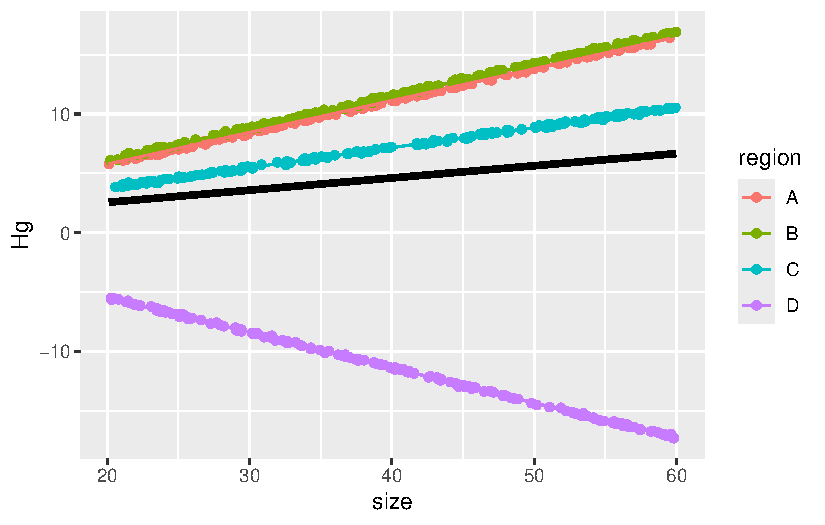
\includegraphics{mixed-effects_files/figure-pdf/unnamed-chunk-15-1.pdf}

\subsection{Answer 3}\label{answer-3}

The intercept and slope significant p-values. This appears to be the
best model.

\begin{tcolorbox}[enhanced jigsaw, title=\textcolor{quarto-callout-important-color}{\faExclamation}\hspace{0.5em}{Question 3. Points:4}, rightrule=.15mm, breakable, colbacktitle=quarto-callout-important-color!10!white, leftrule=.75mm, colback=white, bottomrule=.15mm, toprule=.15mm, opacitybacktitle=0.6, colframe=quarto-callout-important-color-frame, left=2mm, coltitle=black, opacityback=0, bottomtitle=1mm, toptitle=1mm, titlerule=0mm, arc=.35mm]

Re-run the code you used for question 2, but using the new N. Report any
differences that you see after running the model with a low N

\end{tcolorbox}

Total points: 24

Resources:

ggplot cheat sheet:
\url{https://github.com/rstudio/cheatsheets/blob/main/data-visualization.pdf}



\end{document}
